% Options for packages loaded elsewhere
\PassOptionsToPackage{unicode}{hyperref}
\PassOptionsToPackage{hyphens}{url}
%
\documentclass[
]{book}
\usepackage{amsmath,amssymb}
\usepackage{iftex}
\ifPDFTeX
  \usepackage[T1]{fontenc}
  \usepackage[utf8]{inputenc}
  \usepackage{textcomp} % provide euro and other symbols
\else % if luatex or xetex
  \usepackage{unicode-math} % this also loads fontspec
  \defaultfontfeatures{Scale=MatchLowercase}
  \defaultfontfeatures[\rmfamily]{Ligatures=TeX,Scale=1}
\fi
\usepackage{lmodern}
\ifPDFTeX\else
  % xetex/luatex font selection
\fi
% Use upquote if available, for straight quotes in verbatim environments
\IfFileExists{upquote.sty}{\usepackage{upquote}}{}
\IfFileExists{microtype.sty}{% use microtype if available
  \usepackage[]{microtype}
  \UseMicrotypeSet[protrusion]{basicmath} % disable protrusion for tt fonts
}{}
\makeatletter
\@ifundefined{KOMAClassName}{% if non-KOMA class
  \IfFileExists{parskip.sty}{%
    \usepackage{parskip}
  }{% else
    \setlength{\parindent}{0pt}
    \setlength{\parskip}{6pt plus 2pt minus 1pt}}
}{% if KOMA class
  \KOMAoptions{parskip=half}}
\makeatother
\usepackage{xcolor}
\usepackage{color}
\usepackage{fancyvrb}
\newcommand{\VerbBar}{|}
\newcommand{\VERB}{\Verb[commandchars=\\\{\}]}
\DefineVerbatimEnvironment{Highlighting}{Verbatim}{commandchars=\\\{\}}
% Add ',fontsize=\small' for more characters per line
\usepackage{framed}
\definecolor{shadecolor}{RGB}{248,248,248}
\newenvironment{Shaded}{\begin{snugshade}}{\end{snugshade}}
\newcommand{\AlertTok}[1]{\textcolor[rgb]{0.94,0.16,0.16}{#1}}
\newcommand{\AnnotationTok}[1]{\textcolor[rgb]{0.56,0.35,0.01}{\textbf{\textit{#1}}}}
\newcommand{\AttributeTok}[1]{\textcolor[rgb]{0.13,0.29,0.53}{#1}}
\newcommand{\BaseNTok}[1]{\textcolor[rgb]{0.00,0.00,0.81}{#1}}
\newcommand{\BuiltInTok}[1]{#1}
\newcommand{\CharTok}[1]{\textcolor[rgb]{0.31,0.60,0.02}{#1}}
\newcommand{\CommentTok}[1]{\textcolor[rgb]{0.56,0.35,0.01}{\textit{#1}}}
\newcommand{\CommentVarTok}[1]{\textcolor[rgb]{0.56,0.35,0.01}{\textbf{\textit{#1}}}}
\newcommand{\ConstantTok}[1]{\textcolor[rgb]{0.56,0.35,0.01}{#1}}
\newcommand{\ControlFlowTok}[1]{\textcolor[rgb]{0.13,0.29,0.53}{\textbf{#1}}}
\newcommand{\DataTypeTok}[1]{\textcolor[rgb]{0.13,0.29,0.53}{#1}}
\newcommand{\DecValTok}[1]{\textcolor[rgb]{0.00,0.00,0.81}{#1}}
\newcommand{\DocumentationTok}[1]{\textcolor[rgb]{0.56,0.35,0.01}{\textbf{\textit{#1}}}}
\newcommand{\ErrorTok}[1]{\textcolor[rgb]{0.64,0.00,0.00}{\textbf{#1}}}
\newcommand{\ExtensionTok}[1]{#1}
\newcommand{\FloatTok}[1]{\textcolor[rgb]{0.00,0.00,0.81}{#1}}
\newcommand{\FunctionTok}[1]{\textcolor[rgb]{0.13,0.29,0.53}{\textbf{#1}}}
\newcommand{\ImportTok}[1]{#1}
\newcommand{\InformationTok}[1]{\textcolor[rgb]{0.56,0.35,0.01}{\textbf{\textit{#1}}}}
\newcommand{\KeywordTok}[1]{\textcolor[rgb]{0.13,0.29,0.53}{\textbf{#1}}}
\newcommand{\NormalTok}[1]{#1}
\newcommand{\OperatorTok}[1]{\textcolor[rgb]{0.81,0.36,0.00}{\textbf{#1}}}
\newcommand{\OtherTok}[1]{\textcolor[rgb]{0.56,0.35,0.01}{#1}}
\newcommand{\PreprocessorTok}[1]{\textcolor[rgb]{0.56,0.35,0.01}{\textit{#1}}}
\newcommand{\RegionMarkerTok}[1]{#1}
\newcommand{\SpecialCharTok}[1]{\textcolor[rgb]{0.81,0.36,0.00}{\textbf{#1}}}
\newcommand{\SpecialStringTok}[1]{\textcolor[rgb]{0.31,0.60,0.02}{#1}}
\newcommand{\StringTok}[1]{\textcolor[rgb]{0.31,0.60,0.02}{#1}}
\newcommand{\VariableTok}[1]{\textcolor[rgb]{0.00,0.00,0.00}{#1}}
\newcommand{\VerbatimStringTok}[1]{\textcolor[rgb]{0.31,0.60,0.02}{#1}}
\newcommand{\WarningTok}[1]{\textcolor[rgb]{0.56,0.35,0.01}{\textbf{\textit{#1}}}}
\usepackage{longtable,booktabs,array}
\usepackage{calc} % for calculating minipage widths
% Correct order of tables after \paragraph or \subparagraph
\usepackage{etoolbox}
\makeatletter
\patchcmd\longtable{\par}{\if@noskipsec\mbox{}\fi\par}{}{}
\makeatother
% Allow footnotes in longtable head/foot
\IfFileExists{footnotehyper.sty}{\usepackage{footnotehyper}}{\usepackage{footnote}}
\makesavenoteenv{longtable}
\usepackage{graphicx}
\makeatletter
\def\maxwidth{\ifdim\Gin@nat@width>\linewidth\linewidth\else\Gin@nat@width\fi}
\def\maxheight{\ifdim\Gin@nat@height>\textheight\textheight\else\Gin@nat@height\fi}
\makeatother
% Scale images if necessary, so that they will not overflow the page
% margins by default, and it is still possible to overwrite the defaults
% using explicit options in \includegraphics[width, height, ...]{}
\setkeys{Gin}{width=\maxwidth,height=\maxheight,keepaspectratio}
% Set default figure placement to htbp
\makeatletter
\def\fps@figure{htbp}
\makeatother
\setlength{\emergencystretch}{3em} % prevent overfull lines
\providecommand{\tightlist}{%
  \setlength{\itemsep}{0pt}\setlength{\parskip}{0pt}}
\setcounter{secnumdepth}{5}
\usepackage{booktabs}
\usepackage{amsthm}
\makeatletter
\def\thm@space@setup{%
  \thm@preskip=8pt plus 2pt minus 4pt
  \thm@postskip=\thm@preskip
}
\makeatother
\ifLuaTeX
  \usepackage{selnolig}  % disable illegal ligatures
\fi
\usepackage[]{natbib}
\bibliographystyle{apalike}
\IfFileExists{bookmark.sty}{\usepackage{bookmark}}{\usepackage{hyperref}}
\IfFileExists{xurl.sty}{\usepackage{xurl}}{} % add URL line breaks if available
\urlstyle{same}
\hypersetup{
  pdftitle={Introduction to R},
  pdfauthor={Ryan Donovan},
  hidelinks,
  pdfcreator={LaTeX via pandoc}}

\title{Introduction to R}
\author{Ryan Donovan}
\date{2024-01-28}

\begin{document}
\maketitle

{
\setcounter{tocdepth}{1}
\tableofcontents
}
\hypertarget{introduction}{%
\chapter{Introduction}\label{introduction}}

This set of workshops describes how to use R to import, clean, and process psychological data. All materials, data, and information in these workshops are used for educational purposes only. This document should only be shared within the University of Galway's School of Psychology and is not intended for widespread dissemination. The workshop's e-book is very much in its draft stages and will be updated and fine-tuned in the future. Several materials are adapted from various online resources on teaching R.

\hypertarget{who-is-this-resource-for}{%
\section{Who is this resource for?}\label{who-is-this-resource-for}}

These workshops are designed to help people who come from a psychology or social science background learn the necessary programming skills to use R effectively in their research. These workshops are intended for individuals with no programming experience whatsoever, teaching the necessary programming skills and ideas required to conduct statistical techniques in psychology (e.g., Power Analyses, Correlation, ANOVA, Regression, Mediation, Moderation).

These workshops are \textbf{not} for people interested in learning about statistical theory or the who, what, where's of any of the aforementioned statistical techniques. I want these workshops to focus entirely on how to perform statistical analyses in R; I assume you know the rest or know how to access that information.

\hypertarget{should-i-learn-r}{%
\section{Should I learn R?}\label{should-i-learn-r}}

There are many reasons to learn R.

Psychological research is increasingly moving towards open-science practices. One of the key principles of open-science is that all aspects of data handling - including data wrangling, pre-processing, processing, and output generation - are openly accessible. This is not only an abstract want or desire; several top-tier journals require that you submit R scripts along with any manuscripts. If you don't know how to use R (or at least no one in your lab does), then this will put you at a disadvantage.

R enables you to import, clean, analyze, and publish manuscripts from R itself. You do not have to switch between SPSS, Excel, and Word or any other software. You can conduct your statistical analysis directly in R and have that ``uploaded'' directly to your manuscript. In the long run, this will save you so much time and energy.

R is capable of more than statistical analysis. You can create websites, documents, and books in R. This workshop textbook was developed in R! While these initial workshops will not be discussing how to do this (although it is something that I would like to do in the future), I wanted to mention it as an example of how powerful R can be.

\hypertarget{what-will-i-learn-to-do-in-r}{%
\section{What will I learn to do in R?}\label{what-will-i-learn-to-do-in-r}}

The following workshops will teach you how to conduct statistical analysis in R.

R is a statistical programming language that enables you to wrangle, process, and analyze data. By the end of these workshops, you should be able to import a data file into R, do some processing and cleaning, compute descriptive and inferential statistics, generate nice visualizations, and output your results.

The learning objectives of this course are:

\begin{itemize}
\tightlist
\item
  Learn how to import and create datasets in R.
\item
  Learn and apply basic programming concepts such as data types, functions, and loops.
\item
  Learn key techniques for data cleaning in R to enable statistical analysis.
\item
  Learn how to create APA-standard graphs in R.
\item
  Learn how to deal with errors or bugs with R code.
\item
  Learn how to export data.
\end{itemize}

\hypertarget{what-will-i-not-learn-to-do-in-r}{%
\section{What will I not learn to do in R?}\label{what-will-i-not-learn-to-do-in-r}}

This is not an exhaustive introduction to R. Similar to human languages, programming languages like R are vast and will take years to master. After this course, you will still be considered a ``newbie'' in R. But the material covered here will at least provide you a solid foundation in R, enabling you to go ahead and pick up further skills if required as you go on.

This course will teach you data cleaning and wrangling skills that will enable you to wrangle and clean a lot of data collected on Gorilla or Qualtrics. But you will not be able to easily handle all data cleaning problems you are likely to find out in the ``wild'' world of messy data. Such datasets can be uniquely messy, and even experienced R programmers will need to bash their head against the wall a few times to figure out a way to clean that dataset entirely in R. If you have a particularly messy dataset, you might still need to use other programs (e.g., Excel) to clean it up first before importing it to R.

Similarly, do not expect to be fluent in the concepts you learn here after these workshops. It will take practice to become fluent. You might need to refer to these materials or look up help repeatedly when using R on real-life datasets. That's normal.

This workshop is heavily focused on the tidyverse approach to R. The tidyverse is a particular philosophical approach to how to use R (more on that later). The other approach would be to use base R. This can incite violent debates in R communities on which approach is better. We will focus mainly on tidyverse and use some base R.

This workshop does not teach you how to use R Markdown. R Markdown is a package in R that enables you to write reproducible and dynamic reports with R that can be converted into Word documents, PDFs, websites, PowerPoint presentations, books, and much more. That will be covered in the intermediate workshop program.

\hypertarget{where-and-when-will-the-workshops-take-place}{%
\section{Where and when will the workshops take place?}\label{where-and-when-will-the-workshops-take-place}}

The sessions will take place in \textbf{AMB-G035} (Psychology PC Suite). The schedule for the sessions is as follows:

\begin{itemize}
\tightlist
\item
  Feb 7th: Introduction to R and RStudio
\item
  Feb 14th: Basic Programming (Part I)
\item
  Feb 21st: Basic Programming (Part II)
\item
  Feb 28th: Data Cleaning in R (Part I)
\item
  March 6th: Data Cleaning in R (Part II)
\item
  March 13th: Data Visualization
\item
  March 20th: Running Inferential Statistical Tests in R (Part I)
\item
  March 27th: Running Inferential Statistical Tests in R (Part II)
\end{itemize}

Each session is on a Wednesday and will run between 11:00 - 13:00.

\hypertarget{are-there-any-prerequisites-for-taking-this-course}{%
\section{Are there any prerequisites for taking this course?}\label{are-there-any-prerequisites-for-taking-this-course}}

None at all. This course is beginner-friendly. You also do not need to purchase anything (e.g., textbooks or software).

\hypertarget{do-i-need-to-bring-a-laptop-to-the-class}{%
\section{Do I need to bring a laptop to the class?}\label{do-i-need-to-bring-a-laptop-to-the-class}}

If you have a laptop that you work on, I strongly encourage you to bring it. That way, we can get R and RStudio installed onto your laptop, and you'll be able to run R outside of the classroom.

If you work with a desktop, don't worry. The lab space will have computers that you can sign in and work on and use R.

\hypertarget{rstudio}{%
\chapter{Getting Started with R and RStudio}\label{rstudio}}

This workshop introduces the programming language R and the RStudio application. Today, we will download both R and RStudio, set up our RStudio environment, and write and run our first piece of R Code. This will set us up for the rest of the workshops.

\hypertarget{what-actually-is-r}{%
\section{What actually is R?}\label{what-actually-is-r}}

R is a statistical programming language that enables us to directly ask our computer to carry out tasks. Typically, when we use our computers, we do not speak to it directly; instead we interact with ``translators'' (i.e., applications like SPSS), via button-click interfaces, to speak to our computer on our behalf. Such interfaces record and translate our instructions to our computers, who then carry out the instructions and return the results to the application, which then translates those results back to us.

Applications like SPSS are convenient. They usually have a user-friendly button-click based interface and take away the heavy lifting of communicating with our computer. This makes them significantly easier to learn in the short term compared to programming languages.

However, these apps also limit what we can do. For example, base SPSS is functional when it comes to creating visualizations, but it is difficult make major changes to your graph (e.g., making it interactive). If we want to create such visualizations, we will likely need to look elsewhere for it. Similarly, we might also be financially limited in our ability to use such apps, as proprietary software like SPSS is not cheap (\href{https://www.ibm.com/products/spss-statistics/pricing}{it can cost between \$3830 - 25200 for a single licence depending on the version})!

In contrast, R is a free, open-source statistical programming language that enables us to conduct comprehensive statistical analysis and create highly elegant visualizations. By learning R we can cut out the middle man.

\begin{figure}
\centering
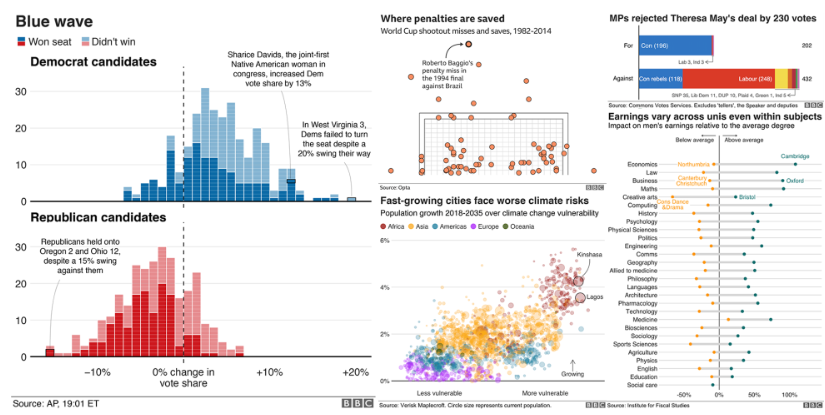
\includegraphics{img/01-bbc.png}
\caption{\label{fig:unnamed-chunk-1}BBC graphs created in R.}
\end{figure}

But why should we learn R and not a different programming language? In contrast to other programming languages (Python, JavaScript, C), R was developed by statisticians. Consequently, R contains an extensive vocabulary to enable us to carry out sophisticated and precise statistical analysis. I have used R and Python to conduct statistical analysis and anytime I wanted to use a less frequently used statistical test, there was significantly more support and information on how to conduct that analysis in R than in Python. For such reasons, R is typically used among statisticians, social scientists, data miners, and bioinformaticians - and will be used in this course\footnote{There are always tradeoffs in selecting a language. Many programming concepts are easier to grasp in Python than in R. Similarly, there is a lot of resources available for conducting machine-learning analysis in Python.

  But if you are goal is conduct data cleaning, analysis, visualization, and reporting, then R is a excellent choice. The good thing is that once you achieve a certain level of competency in one programming language, you will find it significantly easier to pick up a following one.}.

\hypertarget{downloading-r}{%
\section{Downloading R}\label{downloading-r}}

Please follow the following instructions to download R on either Windows or Mac.

\hypertarget{downloading-r-on-windows}{%
\subsection{Downloading R on Windows}\label{downloading-r-on-windows}}

\begin{enumerate}
\def\labelenumi{\arabic{enumi}.}
\tightlist
\item
  Go to the website: \url{https://cran.r-project.org/}
\item
  Under the heading \emph{Download and Install R,} click \emph{Download R for Windows} 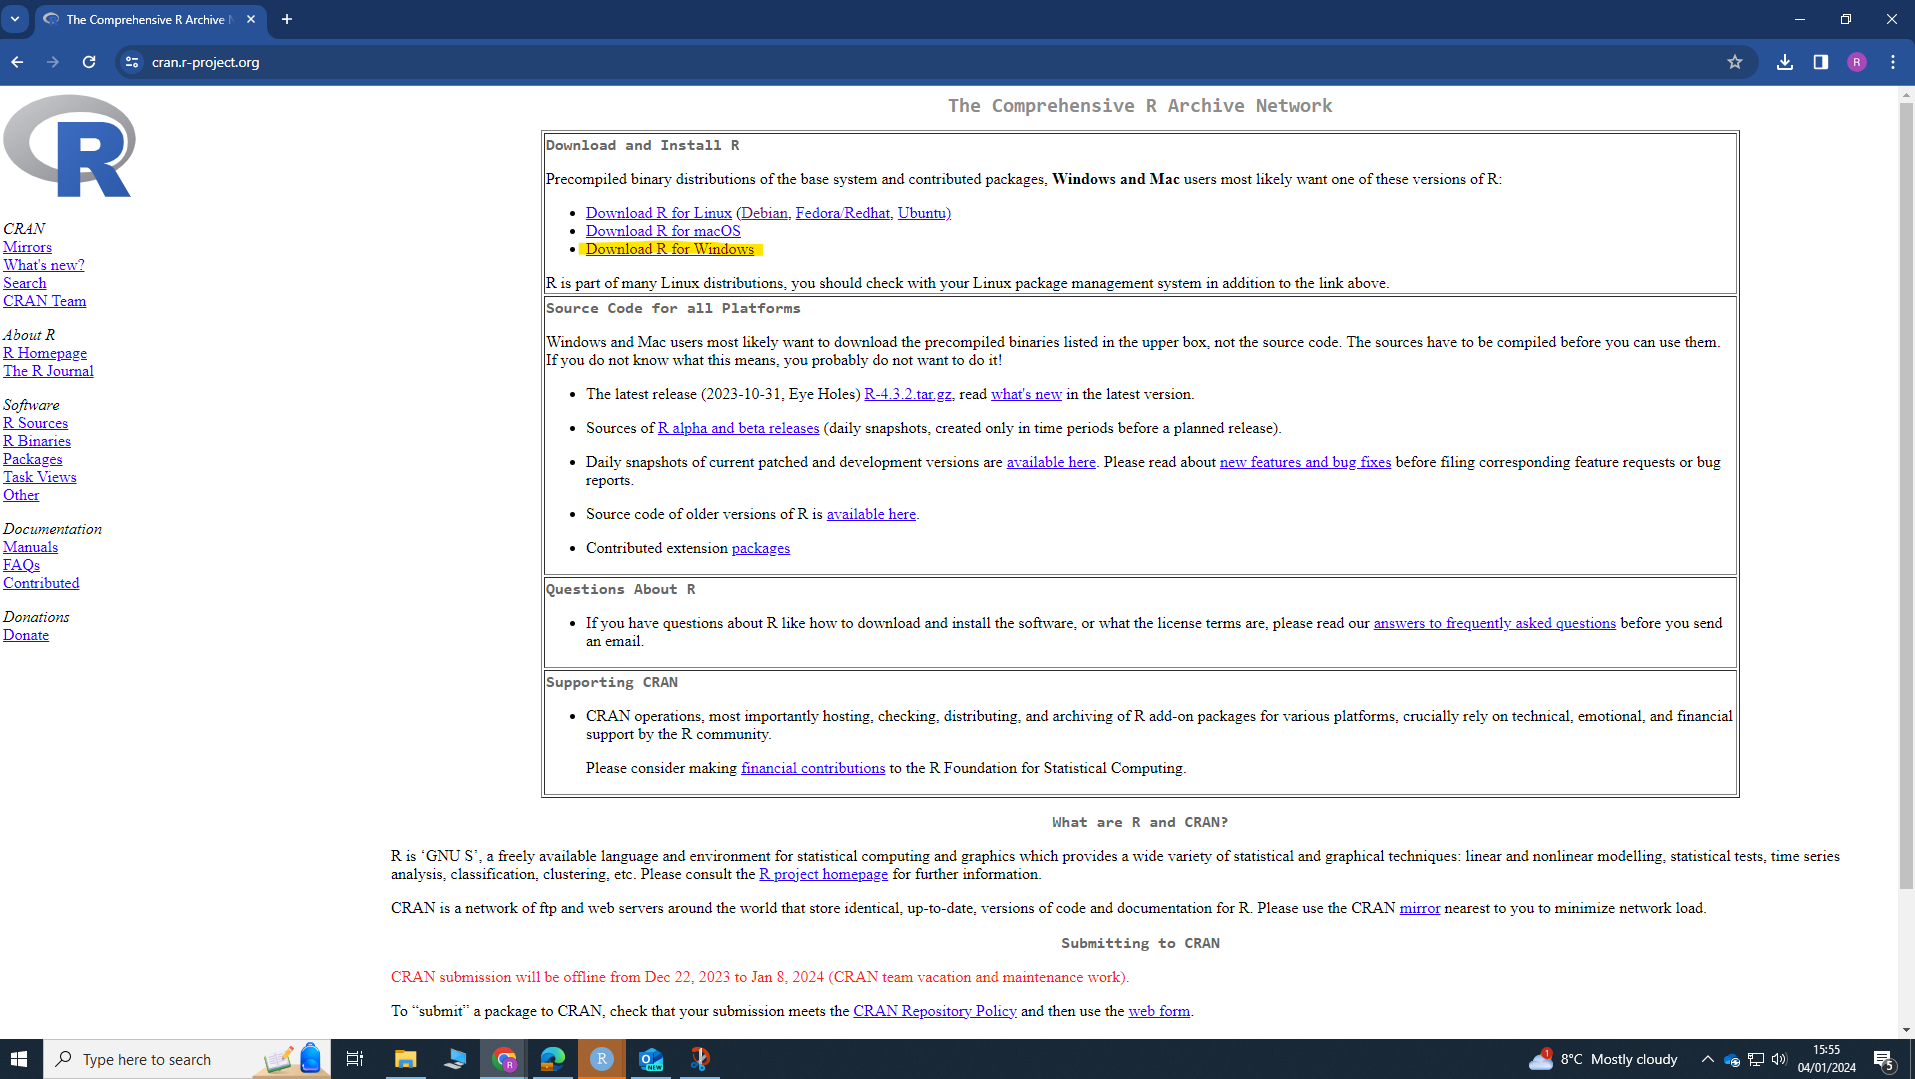
\includegraphics[width=29.20833in,height=\textheight]{img/01-cran.png}
\item
  Click the hyperlink \textbf{\emph{base}} or \textbf{\emph{install R for the first Time}}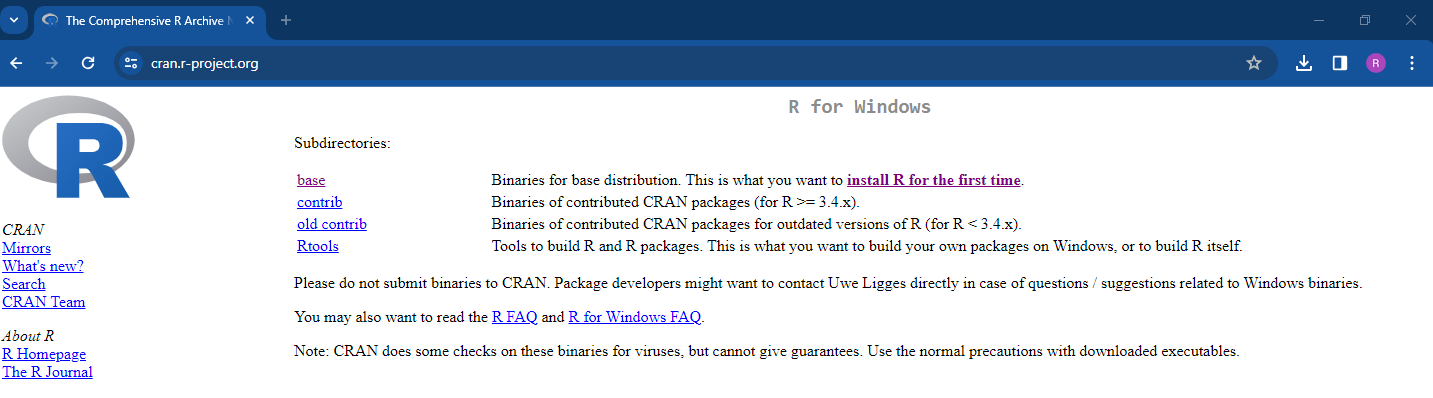
\includegraphics{img/01-base.png}
\item
  Click Download R-4.3.2 for Windows (depending on the date you accessed this, the version of R might have been been updated. That's okay, you can download newer versions). Let the file download. 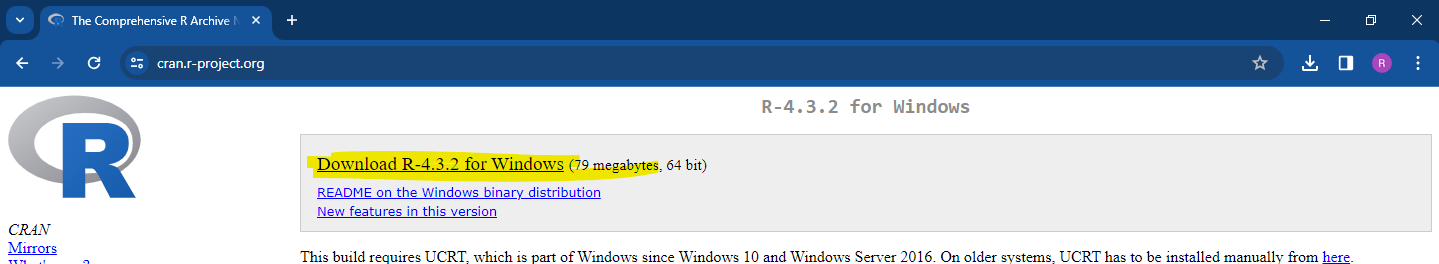
\includegraphics{img/01-download.png}
\item
  Once the file has been downloaded, open it, and click ``Yes'' if you are asked to allow this app to make changes to your device. Then choose English as your setup language. The file name should be something like ``R-4.3.2.-win''. The numbers will differ depending on the specific version that was downloaded.
\item
  Agree to the terms and conditions and select a place to install R. It is perfectly fine to go with the default option.
\end{enumerate}

\hypertarget{downloading-r-on-mac}{%
\subsection{Downloading R on Mac}\label{downloading-r-on-mac}}

The instructions are largely the same for Windows. Please see this guide for more information \url{https://teacherscollege.screenstepslive.com/a/1135059-install-r-and-r-studio-for-mac}

\hypertarget{install-and-open-r-studio}{%
\section{Install and Open R Studio}\label{install-and-open-r-studio}}

Once R is installed, we will install RStudio.

RStudio is a front-end program that makes it it much more user-friendly to use R without sacrificing our ability to code in R. R Studio will enable us to write and save R code, generate plots, manage our files, and do other useful things. RStudio relationship to R is similar to the relationship between a basic text editor and Microsoft Word. We could write a paper in a text editor, but it is much quicker and more efficient to use Word.

\begin{enumerate}
\def\labelenumi{\arabic{enumi}.}
\tightlist
\item
  \textbf{NB:} Make sure that R is installed \textbf{\emph{before}} trying to install R Studio.
\item
  Go to the RStudio website: \url{https://posit.co/download/rstudio-desktop/}
\item
  The website should automatically detect your operating system. Click the \textbf{\emph{Download RStudio Desktop}} button. 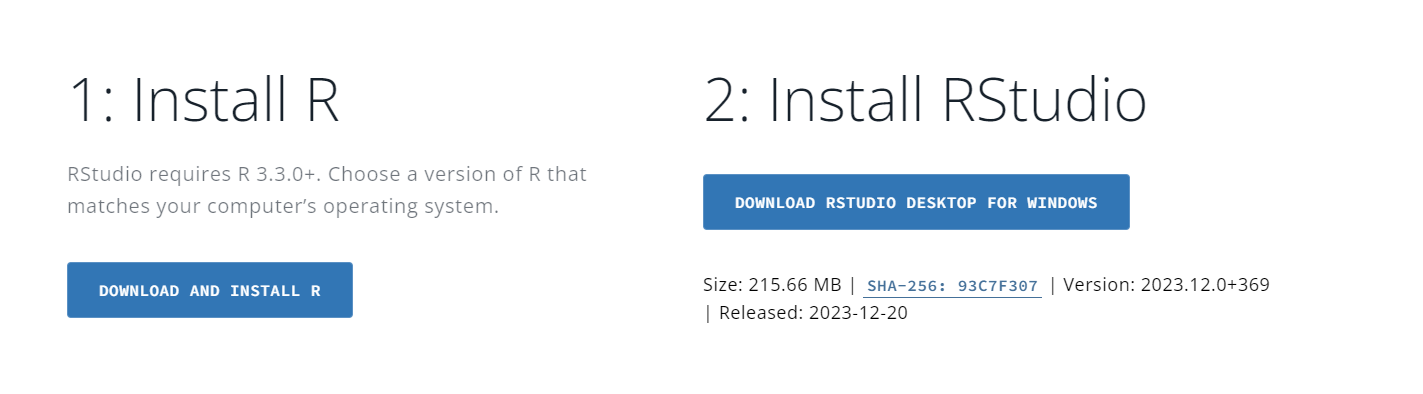
\includegraphics[width=7.1875in,height=\textheight]{img/01-rstudiodownload.png}
\end{enumerate}

Once the file is downloaded, open it and allow it to make changes to your device. Then follow the instructions to download the program. I recommend going with all default options here.

After downloading both R and RStudio, open RStudio on your computer. You do not have to open R as RStudio will work with R (if everything is working correctly).

When you first open RStudio, you will see three panes or ``windows'' in R Studio: ``Console'' (left) ``Environment'' (top right), and ``Files'' (bottom right).

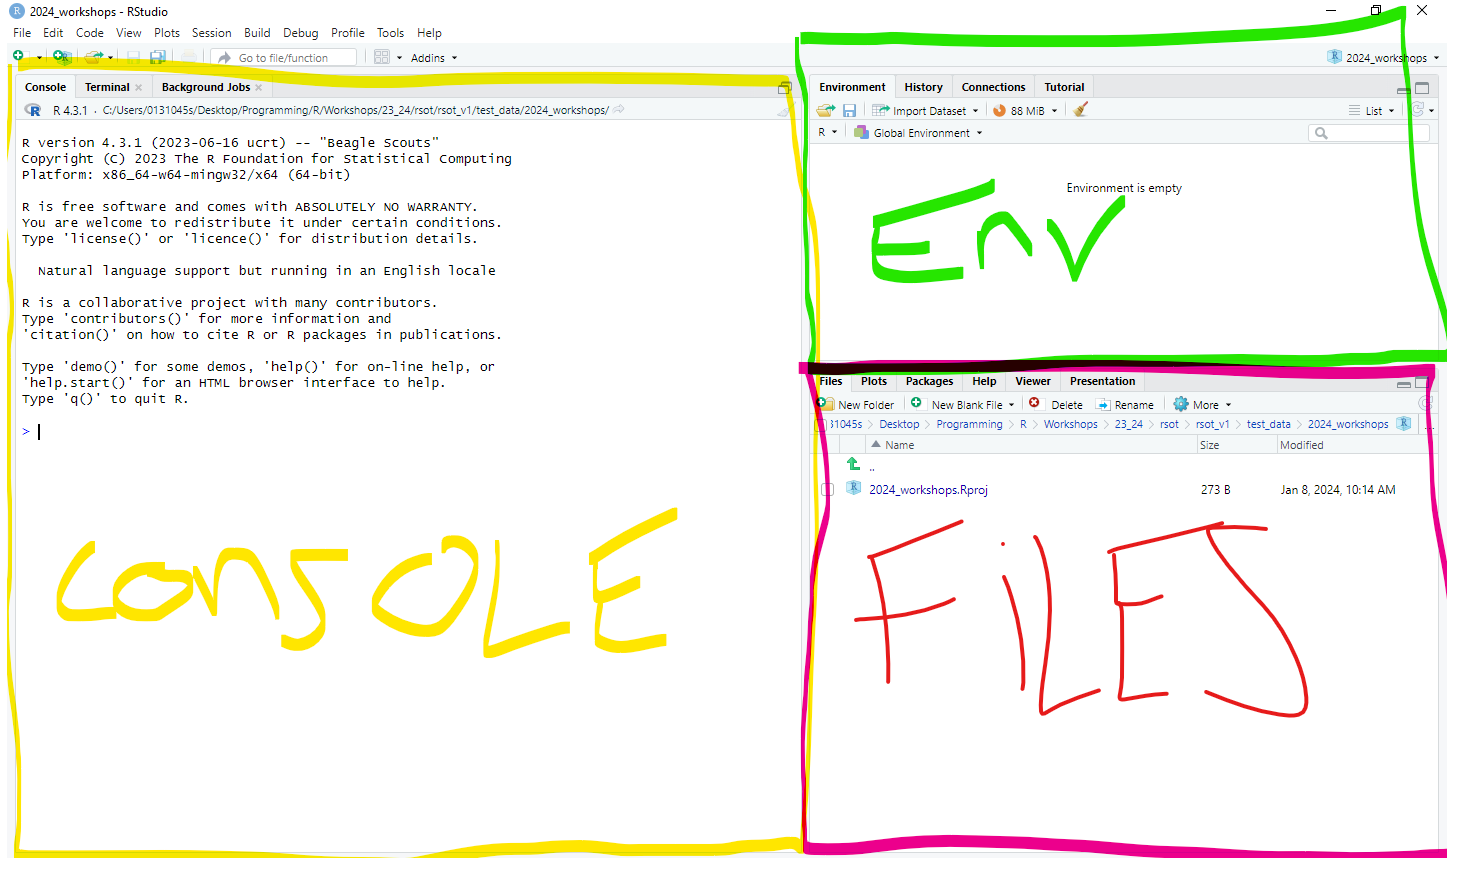
\includegraphics{img/rstudio_first.png}

\hypertarget{creating-an-r-project}{%
\section{Creating an R Project}\label{creating-an-r-project}}

The first thing we will do in RStudio is create a \emph{R Project}. R Projects are environments that will group together input files (e.g., data sets), analyses on those files (e.g., code), and any outputs (e.g., results or plots). Creating an R Project will set up a new directory (folder) on your computer. Any time you open that project, you are telling R to work within this particular directory.

\textbf{\emph{Activity}}

Let's create an R Project that we will use during these workshops.

\begin{enumerate}
\def\labelenumi{\arabic{enumi}.}
\item
  Click ``File'' in the top left hand corner of RStudio-\textgreater{} then click new ``New Project''
\item
  The ``New Project Wizard'' screen will pop up. Click ``New Directory'' -\textgreater{} ``New Project''
\item
  In the ``Create New Project'' screen, there are four options.
\end{enumerate}

\textbf{Option 1}: The ``Directory name'' options sets the name of the project and associated folder.

\begin{itemize}
\item
  You can set this to whatever you want. \textbf{\emph{Just don't set it to ``R'',}} as this can create problems down the line.
\item
  I \textbf{\emph{recommend}} that you set the same directory name as me - \textbf{\emph{introR\_2024}}
\end{itemize}

\textbf{Option 2}: The ``Create project as sub-directory of'' option selects a place to store this project on your computer.

\begin{itemize}
\item
  You can save this anywhere else you like (e.g., your Desktop). Just make sure to save somewhere you can find and somewhere that will not change location (e.g., if you save folders to your desktop, but then tend to move them elsewhere once it gets cluttered, then do not save it to your desktop).
\item
  My recommendation would be to create a folder called ``R\_Programming'' on your desktop. And then save your project in this folder.
\item
  Regardless of where you save your project, copy the location and paste it somewhere you can check (e.g., into a text file)
\end{itemize}

\textbf{Option 3}: The ``Use renv with this project'' option enables you to create a virtual environment for this project that will be separate to other R projects. Don't worry for now about what that means, it will be explained later on.

\begin{itemize}
\tightlist
\item
  Tick this option.
\end{itemize}

\textbf{Option 4:} The ``Open in new session'' just opens a new window on RStudio for this project.

\begin{itemize}
\tightlist
\item
  Tick this option.
\end{itemize}

You can see my example below. Once you're happy with your input for each option, click ``Create Project'' This will open up the project introR\_2024.

\begin{figure}
\centering
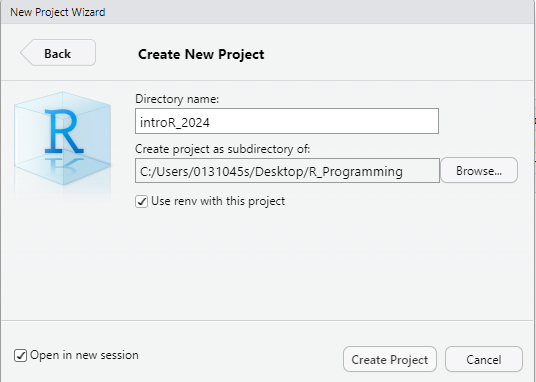
\includegraphics{img/01-newproject.png}
\caption{\label{fig:unnamed-chunk-2}New Project Set Up}
\end{figure}

\hypertarget{navigating-rstudio}{%
\subsection{Navigating RStudio}\label{navigating-rstudio}}

In our new project, introR\_2024, we are going to open the ``Source'' pane, which we will often use for writing code, and viewing datasets.

There are a variety of ways to open the Source pane.

\textbf{Button approach}: Click the ``File'' tab in the top-left hand corner (not the File pane) -\textgreater{} Click ``New File'' -\textgreater{} ``R Script''

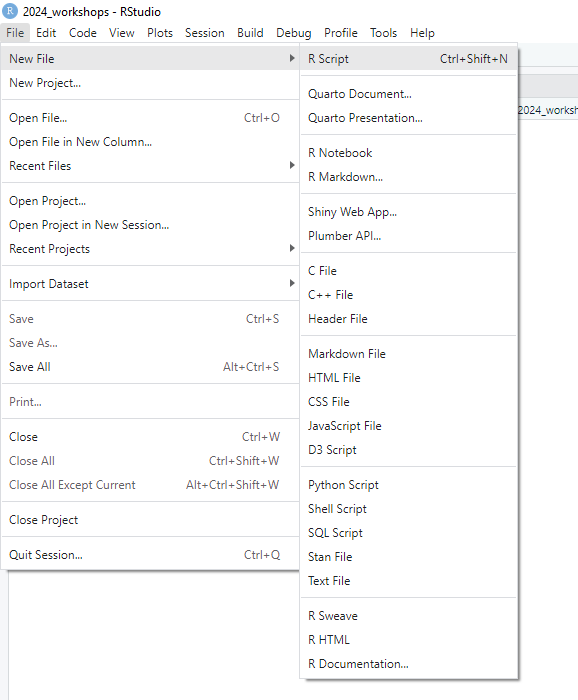
\includegraphics{img/rstudio_create_file.png}

\textbf{\emph{Button Shortcut}}: directly underneath the \emph{File} tab, there is an icon of a white sheet with a green and white addition symbol. You can click that too.

\textbf{Keyboard Shortcut:} You can press ``Ctrl'' + ``Shift'' and ``N'' on Windows. Or ``Cmd'' + ``Shift'' + ``N'' on Mac.

Now you should see your four panes: Source, Console, Environment, and Files.

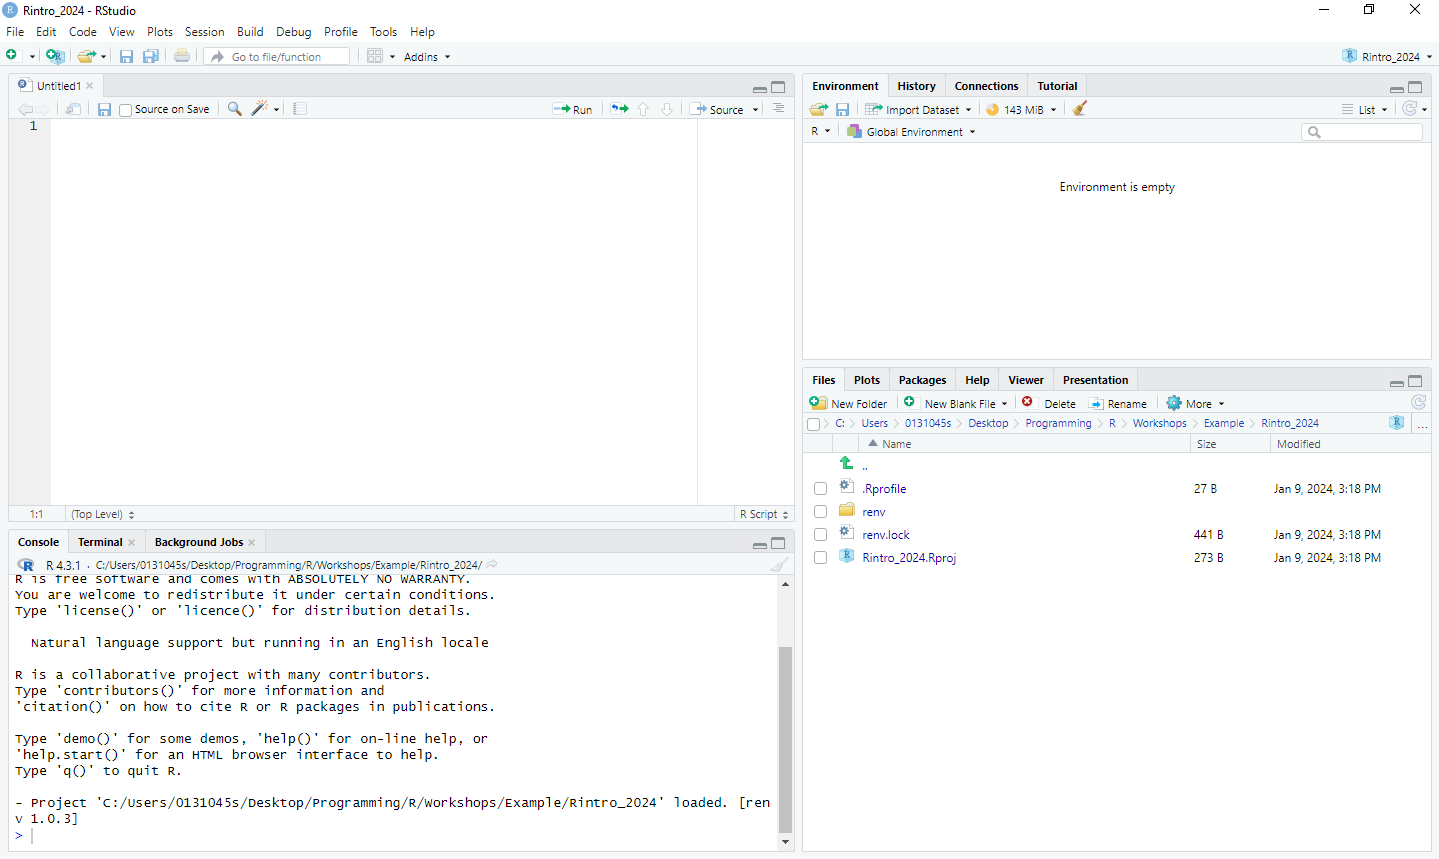
\includegraphics{img/01-four-panes.png}

\hypertarget{the-rstudio-workspace}{%
\subsubsection{The RStudio Workspace}\label{the-rstudio-workspace}}

Now that we have each pane opened, let's briefly describe what each pane is for.

\begin{itemize}
\item
  The \textbf{\emph{Source Pane}} is where you will write R scripts. R scripts enable you to write, save, and run R code in a structured format. For example, you might have an R script titled ``Descriptive'' which contains the code you need to compute descriptive statistics on your data set. Similarly, you might have another R script titled ``Regression'' that contains the code for computing your regression analyses in R.
\item
  The \textbf{\emph{Console Pane}} is where you can write R code or enter commands into R. The console is also where you can find several outputs from your R scripts. For example, if you create a script for running a t-test in R, then the results can be found in the Console Pane. You will also find any error or warning messages about any code that you run (e.g., if you make a mistake in your R code) highlighted in the console. In short, the console is where R is actually running.
\item
  The \textbf{\emph{Environment Pane}} is where you will find information on any data sets and variables that you import or create in R within a bespoke R project. The ``History'' tab will contain a history of any R code that you run during the project. This pane is really useful for getting a bird-eye's view of a project (which can be really useful if you are returning to a project after a long period of time or you are looking at someone's else code).
\item
  The \textbf{\emph{Files Pane}} is where you find your R project files (in the Files tab), the output of any plots that you create (Plots tab), the status of any downloaded packages (Packages tab), and information and helpful information about R functions and packages (Help).
\end{itemize}

Each pane will be used extensively during these workshops.

\hypertarget{checking-our-working-directory}{%
\subsection{Checking our Working Directory}\label{checking-our-working-directory}}

Everytime you open up a project or file in RStudio, it is good practice to check the working directory. The working directory is the environment on our computer that R is currently operating in.

You want the working directory to be in the same location as your R project. That way any files you import into RStudio or any files you export (datasets, results, graphs) can easily be found in your R project folder. A lot of problems can be avoided in R by making sure that you check the working directory. To check the working directory, type the following into the console pane

\begin{Shaded}
\begin{Highlighting}[]
\FunctionTok{getwd}\NormalTok{()}
\end{Highlighting}
\end{Shaded}

\begin{verbatim}
## [1] "/Users/ryandonovan 1/Desktop/Teaching/R/rintro"
\end{verbatim}

What you get in return is the current working directory R is working in. Your working directory will not be the same as mine, that's perfectly normal. Just check to make sure that is in the same location you specified when you created your project (\textbf{Option 2}).

\hypertarget{set_wd}{%
\subsection{Setting up a new Working Directory}\label{set_wd}}

We are going to slightly change our working directory. In our R Project, we are going to create a folder for week1 of the workshop. Anything that we create in R will then be saved into this week1 folder.

\begin{itemize}
\tightlist
\item
  Click ``Session'' on your RStudio toolbar -\textgreater{} Set Working Directory -\textgreater{} Choose Directory
\end{itemize}

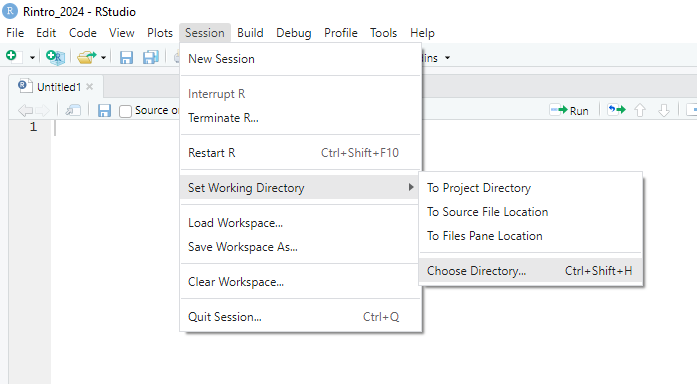
\includegraphics{img/01-wd.png}

\begin{itemize}
\item
  By default you should be in your R Project (e.g., Rintro\_2024).
\item
  Within this R Project, create a new folder and call it ``week1''
\item
  Click ``week1'' and then click Open
\end{itemize}

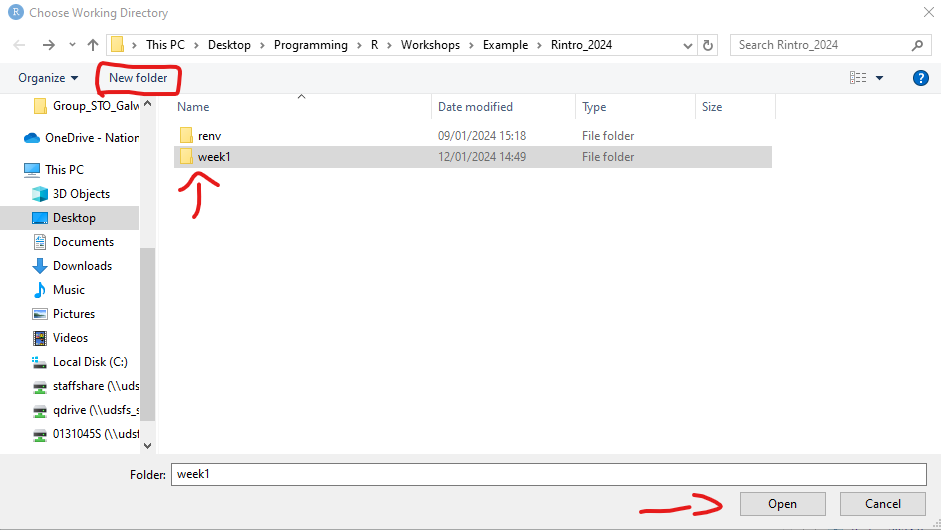
\includegraphics{img/01-new_wd.png}

You should see something like the following in your console

\begin{verbatim}
> setwd("C:/Users/0131045s/Desktop/Programming/R/Workshops/Example/Rintro_2024/week1")
\end{verbatim}

Check whether this is actually the location you want to store your files for this course. If it is, we are good to go. If not, then let me know.

\hypertarget{writing-our-first-r-code}{%
\section{Writing our first R Code}\label{writing-our-first-r-code}}

Let's write our first line of R code in the \textbf{\emph{console}}. The R console uses the operator ``\textgreater{}'' to indicate that it is ready for a new line of code.

Type in the each of the following instructions (after the ´\textgreater´ operator) and press enter. Feel free to change the second line of code to add your own name.

\begin{Shaded}
\begin{Highlighting}[]
\FunctionTok{print}\NormalTok{(}\StringTok{"Hello World"}\NormalTok{)}
\end{Highlighting}
\end{Shaded}

\begin{verbatim}
## [1] "Hello World"
\end{verbatim}

\begin{Shaded}
\begin{Highlighting}[]
\FunctionTok{print}\NormalTok{(}\StringTok{"My name is Ryan and I am learning to code in R"}\NormalTok{)}
\end{Highlighting}
\end{Shaded}

\begin{verbatim}
## [1] "My name is Ryan and I am learning to code in R"
\end{verbatim}

Congratulations, you've written your first piece of code!

Let's describe what is going on here. We used a function called \texttt{print()} to print the words ``Hello World'' and ``My name is Ryan and I am learning to code in R'' in the console. Functions are equivalent to verbs in English language - they describe doing things. In this case, R sees the function print - then it looks inside the bracket to see what we want to print, and then it goes ahead and prints it. Pretty straightforward.

Functions are a very important programming concept, and there is a lot more going on under the hood than I have described so far - so we will be returning to functions repeatedly and filling you in with more information. But in essence functions are verbs that enable us to tell our computer to carry out specific actions on objects.

\hypertarget{console-vs-source-script}{%
\section{Console vs Source Script}\label{console-vs-source-script}}

You might have noticed that I asked you to write code in the console rather than in the source pane. It's worth discussing here what the differences are between the console and the script when it comes to writing code.

The console is like the immediate chat with R. It's where you can type and execute single lines of code instantly. Imagine it as a friendly conversation where you ask R to do something, and it responds right away. The console The console is fantastic for experimenting and getting instant feedback. It's your interactive playground, perfect for spontaneous interactions with R.

The console is also really useful for performing quick calculations, testing functions or pieces of code, and for running code that should run once and only once.

However, the console is cumbersome to use if we want to write code that is several lines long and/or when we want to structure or save our code. This is where R scripts come in.

R scripts are text files where we can write R code in a structured manner. Scripts enable us to structure our code (e.g., with headings and instructions), write several pieces of code, and save and rerun code easily. If you think of your console as a draft, then your script is for the code that you want to keep.

From now on, whenever we write code, we are going to be using R scripts by default. For the times we will write code in the console, I will let you know beforehand.

\hypertarget{lets-write-some-statistical-code}{%
\section{Let's write some statistical code}\label{lets-write-some-statistical-code}}

Okay we have talked a lot about R and RStudio. To finish off this session, let's write code that will take a data set, calculate some descriptive statistics, run an inferential test, generate a graph, and save our results. Don't worry if you do not understand any of the following code. Just follow along and type it yourself in the R script we opened up earlier (if it's not open, click ``File'' -\textgreater{} New File -\textgreater{} RScript). Once you have created this script, save it as ``01-paired-t-tests''.

When you download R, you will have automatic access to several functions (e.g., print) and data sets. One of these data sets are called sleep, which we are going to use right now. To learn more about the sleep data set, type \texttt{?sleep} into the console. You will find more information on the data sets in the Files pane, under the Help tab.

First let's have a look at the sleep data set by writing the following code in the R script. To run scripts in R, select the code you have written and click the Run button with the green arrow in the top right corner of the script.

\begin{Shaded}
\begin{Highlighting}[]
\FunctionTok{print}\NormalTok{(sleep) }
\end{Highlighting}
\end{Shaded}

\begin{verbatim}
##    extra group ID
## 1    0.7     1  1
## 2   -1.6     1  2
## 3   -0.2     1  3
## 4   -1.2     1  4
## 5   -0.1     1  5
## 6    3.4     1  6
## 7    3.7     1  7
## 8    0.8     1  8
## 9    0.0     1  9
## 10   2.0     1 10
## 11   1.9     2  1
## 12   0.8     2  2
## 13   1.1     2  3
## 14   0.1     2  4
## 15  -0.1     2  5
## 16   4.4     2  6
## 17   5.5     2  7
## 18   1.6     2  8
## 19   4.6     2  9
## 20   3.4     2 10
\end{verbatim}

The \texttt{print()} function here prints out the sleep data set in the console. There are also other ways to view a data set, such as using the functions \texttt{head()}, \texttt{tail()} \texttt{View()}, and \texttt{str()}. Type these in the console (make sure to put \texttt{sleep} inside the brackets) and see what results you get.

The result of \texttt{print(sleep)} shows us there are 20 observations in the dataset (rows), with three difference variables (columns): extra (hours of extra sleep each participant had), group (which treatment they were taken), and ID (their participant ID).

Now let's calculate some descriptive statistics. One we can do this is by using the summary() function. This function takes in an an object (e.g., like a data set) and summaries the data. Write the following in your R script and press run.

\begin{Shaded}
\begin{Highlighting}[]
\FunctionTok{summary}\NormalTok{(sleep) }
\end{Highlighting}
\end{Shaded}

\begin{verbatim}
##      extra        group        ID   
##  Min.   :-1.600   1:10   1      :2  
##  1st Qu.:-0.025   2:10   2      :2  
##  Median : 0.950          3      :2  
##  Mean   : 1.540          4      :2  
##  3rd Qu.: 3.400          5      :2  
##  Max.   : 5.500          6      :2  
##                          (Other):8
\end{verbatim}

Running \texttt{summary(sleep)} shows us descriptive statistics for each of our variables. We can see that the mean change in hours of sleep were +1.5, and that there was 10 participants within both the control and experimental condition.

But it's not perfect. Firstly, we don't need summary descriptive on the participant ID. Secondly, it only tells us the mean the entire sample, whereas we are more interested in the mean score per each treatment group. We can get this information by using the \texttt{aggregate()} function, which enables us to split our data into subset and then compute summary statistics per group. Remember to press run after you written your code.

\begin{Shaded}
\begin{Highlighting}[]
\CommentTok{\#The code inside the aggregate bracket tells our computer to: }
\CommentTok{\# data = sleep {-}\textgreater{} Go to the sleep data set}

\CommentTok{\#extra \textasciitilde{} group {-}\textgreater{} Take the variable "extra" and split it into subsets based on the variable "group"}

\CommentTok{\# FUN = mean {-}\textgreater{} Apply the mean() function (FUN) on each subset }

\FunctionTok{aggregate}\NormalTok{(}\AttributeTok{data =}\NormalTok{ sleep, extra }\SpecialCharTok{\textasciitilde{}}\NormalTok{ group, }\AttributeTok{FUN =}\NormalTok{ mean)}
\end{Highlighting}
\end{Shaded}

\begin{verbatim}
##   group extra
## 1     1  0.75
## 2     2  2.33
\end{verbatim}

That's more like it. Now we can see that there does seem to a difference between treatment1 and treatment2. Participants slept an extra 2.33 hours on average when taking treatment 2, whereas they only slept .75 hours (e.g., 45 minutes) more on average when taking treatment 1. So treatment 2 does seem more effective.

Let's run a paired-samples t-test to see if those differences are significant (assuming all parametric assumptions are met, of course\ldots).

\begin{Shaded}
\begin{Highlighting}[]
\FunctionTok{t.test}\NormalTok{(sleep}\SpecialCharTok{$}\NormalTok{extra[sleep}\SpecialCharTok{$}\NormalTok{group }\SpecialCharTok{==} \DecValTok{1}\NormalTok{], }\CommentTok{\#this code extracts the group 1 scores}
\NormalTok{       sleep}\SpecialCharTok{$}\NormalTok{extra[sleep}\SpecialCharTok{$}\NormalTok{group }\SpecialCharTok{==} \DecValTok{2}\NormalTok{], }\CommentTok{\# this code extracts group 2 scores}
       \AttributeTok{paired =} \ConstantTok{TRUE}\NormalTok{) }\CommentTok{\#this code tells R to run a paired t{-}test, not between/independent t{-}test}
\end{Highlighting}
\end{Shaded}

\begin{verbatim}
## 
##  Paired t-test
## 
## data:  sleep$extra[sleep$group == 1] and sleep$extra[sleep$group == 2]
## t = -4.0621, df = 9, p-value = 0.002833
## alternative hypothesis: true mean difference is not equal to 0
## 95 percent confidence interval:
##  -2.4598858 -0.7001142
## sample estimates:
## mean difference 
##           -1.58
\end{verbatim}

Boom! We can see there is a statistically significant difference between the two groups. I know the code within the t-test might look a bit complicated, but we will break it down and explain it as we go on in further weeks.

Finally let's visualize our data with the plot() function.

\begin{Shaded}
\begin{Highlighting}[]
\FunctionTok{plot}\NormalTok{(sleep}\SpecialCharTok{$}\NormalTok{group, sleep}\SpecialCharTok{$}\NormalTok{extra)}
\end{Highlighting}
\end{Shaded}

\begin{figure}
\centering
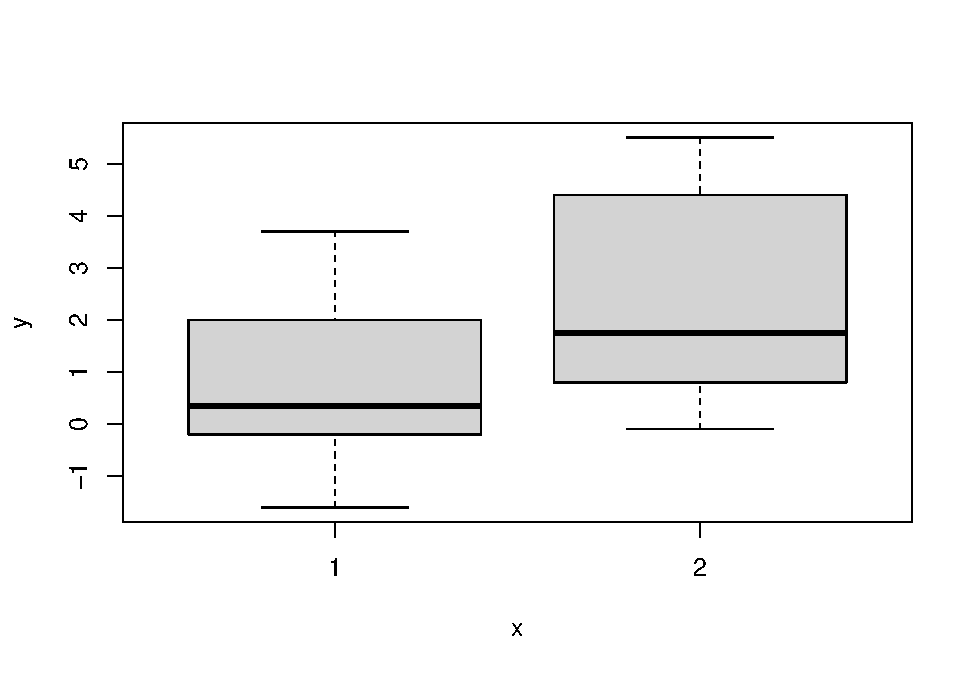
\includegraphics{gitbook-demo_files/figure-latex/unnamed-chunk-8-1.pdf}
\caption{\label{fig:unnamed-chunk-8}Generic Boxplot}
\end{figure}

The plot() function is an example of a generic function, which means it's a function that will try to adapt to our code. In this case, the plot() function looks at the variables we wants to plot, and identifies that the box plot is the most appropriate way to plot it.

Now this plot is perfectly adequate for a first viewing, but let's make it a bit more instructive by adding labels to the x and y axis, and by adding a title to it.

\begin{Shaded}
\begin{Highlighting}[]
\CommentTok{\#xlab = creates a label for the x{-}axis  }

\CommentTok{\#ylab = creates a title for the y{-}axis  }

\CommentTok{\#main = creates a title for the plot  }



\FunctionTok{plot}\NormalTok{(sleep}\SpecialCharTok{$}\NormalTok{group, sleep}\SpecialCharTok{$}\NormalTok{extra, }\AttributeTok{xlab =} \StringTok{"Treatment"}\NormalTok{, }\AttributeTok{ylab =} \StringTok{"Hours of Sleep"}\NormalTok{, }\AttributeTok{main =} \StringTok{"Effect of Treament on Sleep Duration"}\NormalTok{)  }
\end{Highlighting}
\end{Shaded}

\begin{figure}
\centering
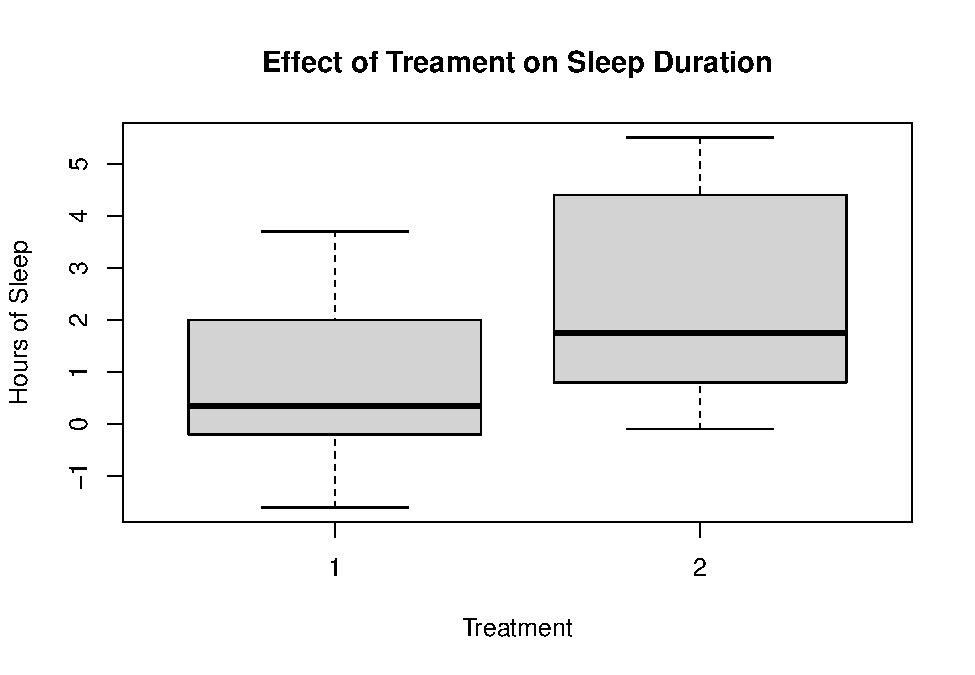
\includegraphics{gitbook-demo_files/figure-latex/unnamed-chunk-9-1.pdf}
\caption{\label{fig:unnamed-chunk-9}Generic Boxplot with appropriate labelling}
\end{figure}

Now let's take this plot and save it to a PDF so that we could share our results with others. The standard way of doing this in R is a bit cumbersome. We have to tell R that we are about to create a plot that we want to make into a PDF. Then we have to generate the plot. Then we have to tell R we are done with creating the PDF. We'll learn a MUCH simpler way to do this in future weeks, but this will do for now.

\begin{Shaded}
\begin{Highlighting}[]
\FunctionTok{pdf}\NormalTok{(}\AttributeTok{file =} \StringTok{"myplot.pdf"}\NormalTok{) }\CommentTok{\#Tells R that we will create a pdf file called "my\_plot" in our working directory}

\FunctionTok{plot}\NormalTok{(sleep}\SpecialCharTok{$}\NormalTok{group, sleep}\SpecialCharTok{$}\NormalTok{extra, }\AttributeTok{xlab =} \StringTok{"Treatment"}\NormalTok{, }\AttributeTok{ylab =} \StringTok{"Hours of Sleep"}\NormalTok{, }\AttributeTok{main =} \StringTok{"Effect of Treament on Sleep Duration"}\NormalTok{)  }\CommentTok{\#this will save the plot to our pdf}


\FunctionTok{dev.off}\NormalTok{() }\CommentTok{\#this tells R that we are done with adding stuff to our PDF}
\end{Highlighting}
\end{Shaded}

\begin{verbatim}
## pdf 
##   2
\end{verbatim}

Go to the files pane, and open up the pdf ``myplot.pdf''. It should be in your working directory. Open it up the PDF and have a look at your graph\footnote{This is a fairly generic type of graph offered by base R. During the course we will looking at ways we can create ``sexier'' and more APA friendly type of graphs. But for one line of code, it's not bad!}.

\hypertarget{comments}{%
\subsection{Comments}\label{comments}}

Last concept before we finish. You might have noticed that I wrote several things with a \texttt{\#} before them. These are known as comments. Comments are any piece of text that will be ignored by R (i.e., they will not be executed within the console). They are fundamental to writing clear code.

We create comments using \texttt{\#} symbol. This symbol tells R to ignore whatever comes directly \textbf{\emph{afterwards}}.

There are various reasons for using comments.

\begin{figure}
\centering
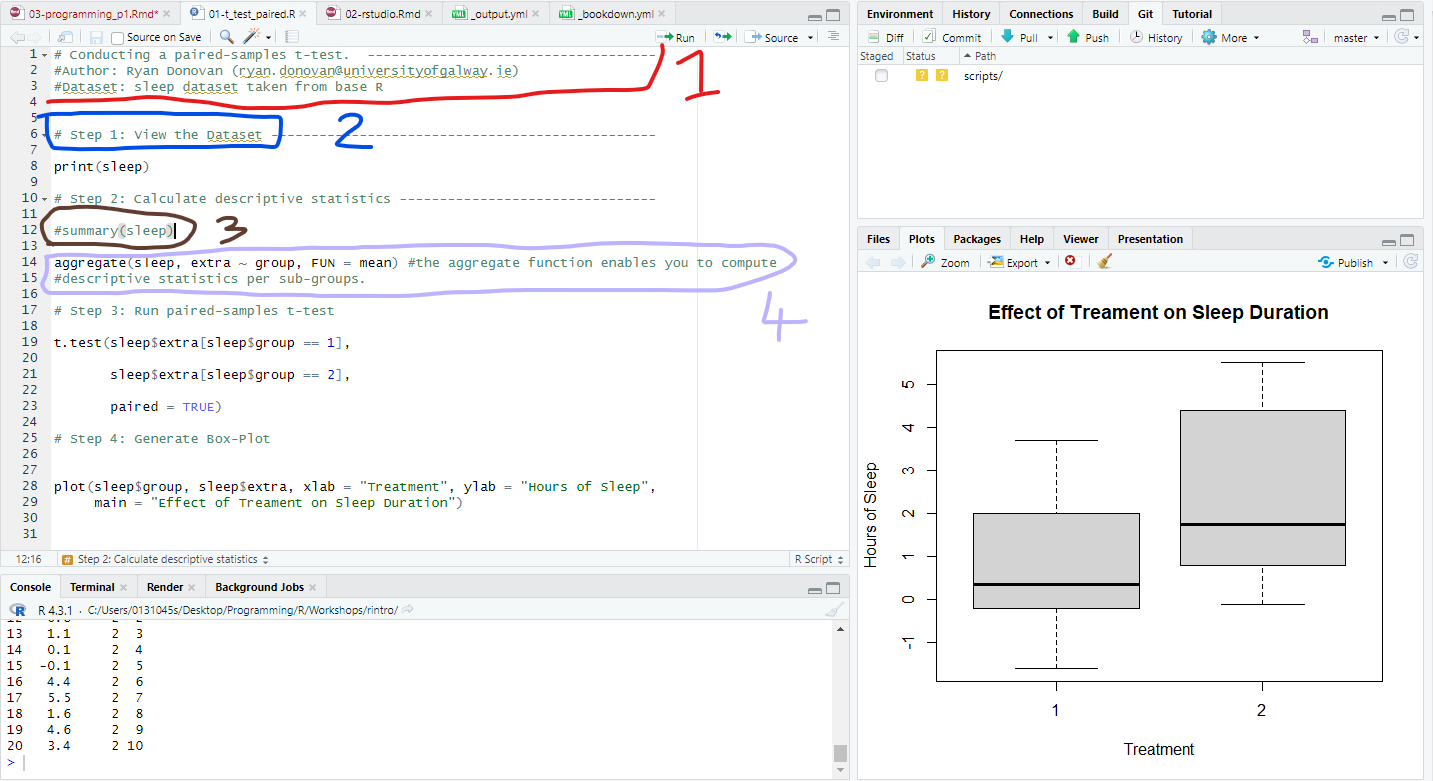
\includegraphics{img/03-comments.png}
\caption{\label{fig:unnamed-chunk-11}Four Examples of Comments Use}
\end{figure}

In the above figure, you'll see four different types of comments.

\begin{enumerate}
\def\labelenumi{\arabic{enumi}.}
\item
  The first type of comment provides a quick introduction to the R script. It can be really useful here to provide a clear information on what this script is trying to do (e.g., run a paired samples t-test), what data it is working on (the sleep dataset), and who wrote or developed this script. This makes it significantly easier for anyone who might be reviewing your work or trying to apply your code to their own work to understand what is going on.
\item
  The second type of comment structures the format of the script by providing headings or steps. Again, this just makes it easier to understand what is going on.
\item
  The third type of comment is placed before the summary. This means that code \texttt{summary(sleep)} will not be executed in R. Why would we do this? If you remember last week, we wanted to compute the mean per each of our two treatment groups, which the summary function does not enable us to do, so it's not part of our main analysis. So why keep it? Well it still provides us with valuable information (e.g., mean, median, min, max for the entire sample), so rather than delete it, we'll just put a comment in front of it. And if anytime we want to check these descriptives, we can just remove the \texttt{\#} and run that line of code.
\item
  The fourth type of comment provides some context or information on what a specific line of code is doing, namely, what the \texttt{aggregate()} function does. Again, this is really useful, particularly if you are using functions that are now well known.
\end{enumerate}

Comments are extremely useful for orientating yourself to code. My advice would be to comment as much as your code as you. Anyone who has coded will have experience the following situation - You spend days/weeks writing a piece of code to clean a messy data set and run a specialized type of analysis. Several months go by and you need to return to your data set (pesky reviewer \#2 wants you change something). You open up your R script and you are \textbf{\emph{completely lost}}. You have written no comments, so you have to spend days trying to remember what each piece of code was trying to do.

If you comment a lot, it will save you so much heartache in the future. And it will help you understand various code concepts better if you can explain them while you are using them. So comment, comment, comment!

\hypertarget{summary}{%
\section{Summary}\label{summary}}

There we have it! That completes our first session with R and RStudio. Today was more about getting to grips with the software R and RStudio, but we still got our first pieces of code written. Hopefully it's given you a tiny glimpse into what R can do.

In the next two sessions, we will learn basic programming concepts and how to import data in R.

\hypertarget{programming1}{%
\chapter{Basic R Programming (Part I)}\label{programming1}}

Today we are going to learn some basic programming concepts. By the end of the session, you should be able to:

\begin{itemize}
\item
  Run and troubleshoot commands in the R console.
\item
  Understand the different data types and when they are used.
\item
  Create and use variables.
\item
  Understand data structures and how to create them.
\item
  Load R packages and use their functions.
\end{itemize}

\hypertarget{activity-1-set-up-your-working-directory}{%
\subsection{Activity 1: Set up your Working Directory}\label{activity-1-set-up-your-working-directory}}

It's good practice to set your working directory when you first open RStudio. Remember that the working directory is the location where we want to store any resulting data files or scripts that you'll work on in a session. Last week I showed you how to do this using \protect\hyperlink{set_wd}{a button-and-click interface}.

Using those instructions, create a folder called ``Week2'' in the \texttt{rintro} project folder and set it as your working directory. Use the ´getwd()´ to check that it has been set as your working directory. Your output should be something like this:

\begin{Shaded}
\begin{Highlighting}[]
\SpecialCharTok{\textgreater{}} \FunctionTok{setwd}\NormalTok{(}\StringTok{"C:/Users/0131045s/Desktop/Programming/R/Workshops/Example/Rintro\_2024/week2"}\NormalTok{)}
\end{Highlighting}
\end{Shaded}

\hypertarget{using-the-console}{%
\section{Using the Console}\label{using-the-console}}

In the previous chapter, I made a distinction between the script and the console. I said that the script was an environment where we would write and run polished code, and the R console is an environment for writing and running ``dirty'' quick code to test ideas, or code that we would run once.

That distinction is kinda true, but it's not completely true. In reality, when we write a script we are preparing \textbf{\emph{commands}} for R to \textbf{\emph{execute}} in the console. In this sense, the R script is equivalent to a waiter. We tell the waiter (script) what we want to order, and then the waiter hands that order to the chef (console).

It's important to know how to work the R console, even if we mostly use scripts in these workshops. We don't want the chef to spit into our food.

\hypertarget{typing-commands-in-the-console}{%
\subsection{Typing Commands in the Console}\label{typing-commands-in-the-console}}

We enter in our code after this operator and press enter to compute it.

We can command the R console to compute calculations. Remember not to type the operator ´\textgreater´ if you are following along in RStudio, this just indicates that R is ready to execute a new command.\footnote{Including the ``\textgreater{}'' is a pain when formatting this book, so I won't include ``\textgreater{}'' in examples of code from this point forward.}

\begin{Shaded}
\begin{Highlighting}[]
\SpecialCharTok{\textgreater{}} \DecValTok{10} \SpecialCharTok{+} \DecValTok{20}

\NormalTok{[}\DecValTok{1}\NormalTok{] }\DecValTok{30}
\end{Highlighting}
\end{Shaded}

\begin{Shaded}
\begin{Highlighting}[]
\SpecialCharTok{\textgreater{}} \DecValTok{20} \SpecialCharTok{/} \DecValTok{10}

\NormalTok{[}\DecValTok{1}\NormalTok{] }\DecValTok{2}
\end{Highlighting}
\end{Shaded}

If you are performing calculations in R, it's important to know that it follows the usual arithmetic convention of order of operations (remember \href{https://www.tes.com/en-ie/teaching-resource/bidmas-bodmas-bedmas-bimdas-pemdas-permdas-11154272\#:~:text=\%E2\%80\%A2\%20BIMDAS\%20\%2D\%20Brackets\%2C\%20Indices\%2C,Multiplication\%2C\%20Division\%2C\%20Addition\%2C\%20Subtraction}{BIMDAS - Bracets, Indices, Multiplication, Division, Addition, and Subtraction?}).

\begin{Shaded}
\begin{Highlighting}[]
\SpecialCharTok{\textgreater{}}\NormalTok{ (}\DecValTok{20} \SpecialCharTok{+} \DecValTok{10} \SpecialCharTok{/} \DecValTok{10}\NormalTok{) }\SpecialCharTok{*} \DecValTok{4} 

\NormalTok{[}\DecValTok{1}\NormalTok{] }\DecValTok{84}

\SpecialCharTok{\textgreater{}}\NormalTok{ ((}\DecValTok{20} \SpecialCharTok{+} \DecValTok{10}\NormalTok{) }\SpecialCharTok{/} \DecValTok{10}\NormalTok{) }\SpecialCharTok{*} \DecValTok{4}

\NormalTok{[}\DecValTok{1}\NormalTok{] }\DecValTok{12}
\end{Highlighting}
\end{Shaded}

Now you'll have noticed that the output of every line of code we entered starts with a \textbf{\texttt{{[}1{]}}} before our actual result. What does this mean?

Think of the square brackets with a number as a way for R to label and organize its responses. Imagine you have a conversation with R, and every time you ask it something, it gives you an answer. The square brackets with a number, like \textbf{\texttt{{[}1{]}}}, are like labels on each response, telling you which answer corresponds to which question. This is R \textbf{\emph{indexing}} its answer.

In each of the above examples, we asked R one question \textbf{\emph{per each}} command, which is why the answer is always \textbf{\texttt{{[}1{]}}}. If we entered longer code with multiple questions, then we could multiple answers. We could tell which answer related to which question through the index. This is really useful when we ask R long and more complicated questions.

\hypertarget{console-syntax-aka-im-ron-burgundy}{%
\subsection{Console Syntax (Aka ``I'm Ron Burgundy?'')}\label{console-syntax-aka-im-ron-burgundy}}

\hypertarget{r-console-and-typos}{%
\subsubsection{R Console and Typos}\label{r-console-and-typos}}

One of the most important concepts you need to understand when you are programming, is that you need to type exactly what you want R to do. If you make a mistake (e.g., a typo), R will not try and understand what you actually meant. For example, see what happens if you make the following mistake:

\begin{Shaded}
\begin{Highlighting}[]
\SpecialCharTok{\textgreater{}} \DecValTok{10} \OtherTok{=} \DecValTok{20}
\end{Highlighting}
\end{Shaded}

\begin{verbatim}
## Error in 10 = 20: invalid (do_set) left-hand side to assignment
\end{verbatim}

R thinks you making the claim that 10 equals 20. Since this is not true, R panics and refuses to run your command. Now any person looking at that code would guess that since \texttt{+} and \texttt{=} are on the same key on our keyboards, the person probably meant to type \texttt{10\ +\ 20}. But we have a strong theory of mind whereas programming languages do not.

So be exact with your code or else be Ron Burgundy(?) \href{https://www.youtube.com/watch?v=X3zfP14pLxc}{a Ron Burgundy situation.}.

This type of mistakes are pretty benign, as R will tell us immediately that something is wrong. However, there can be a more silent type of mistake that can be more damaging. Let's image that you typed in \texttt{-} instead of \texttt{+} by mistake.

\begin{Shaded}
\begin{Highlighting}[]
\SpecialCharTok{\textgreater{}} \DecValTok{10} \SpecialCharTok{{-}} \DecValTok{20}

\NormalTok{[}\DecValTok{1}\NormalTok{] }\SpecialCharTok{{-}}\DecValTok{10}
\end{Highlighting}
\end{Shaded}

In this scenario, R will run this code and output the result. This is because the code still makes sense - it is perfectly legitimate to subtract 20 away from 10. R can't read your mind, so it sees three symbols in a perfectly logical order, and carries out the command. It assumes you're the adult here.

In short calculations like this, it will clear what you typed wrong. However, if you run a long-block of connected code and made a typo like this somewhere, the result you get be significantly different from the intended result. The main way to check for this is to always view the output of your code. If it looks significantly different from what you expected, then this type of silent error might be causing it.

\hypertarget{r-console-and-incomplete-commands}{%
\subsubsection{R Console and Incomplete Commands}\label{r-console-and-incomplete-commands}}

I have been pretty mean to the console, but there are rare times it will be a good Samaritan. For example, if R thinks you haven't finished a command it will print out \texttt{+} to allow you to finish it.

\begin{Shaded}
\begin{Highlighting}[]
\SpecialCharTok{\textgreater{}}\NormalTok{ (}\DecValTok{20} \SpecialCharTok{+} \DecValTok{10}
 
\SpecialCharTok{+}\NormalTok{ )}

\NormalTok{[}\DecValTok{1}\NormalTok{] }\DecValTok{30}
\end{Highlighting}
\end{Shaded}

So when you see ``+'' in the console, this is R telling you that something is missing. If nothing is missing, then this indicates that your code might not be correctly formatted. Overall, the moral of this section can be summarized as: proofread your code!

Okay, that's a lot about using the console. Let's move on to other programming concepts.

\hypertarget{data-types}{%
\section{Data Types}\label{data-types}}

Our overall goal for this course is to give you the ability to import your data into R, select a subset of the data most of interest for a given analysis, carry out an analysis to summarize these data and create visualizations of the data. But it's important to consider \textbf{\emph{What is Data and how is it stored in R?}}

Data comes in many forms: Numbers (Integers and decimal values) or alphabetical (characters or lines of text). R has developed a system for classifying this range of data into different data types.

\hypertarget{basic-data-types-in-r}{%
\section{Basic Data types in R}\label{basic-data-types-in-r}}

R has 4 basic data types that are used 99\% of the time:

\hypertarget{character}{%
\subsection{Character}\label{character}}

A character is anything wrapped inside quotation marks. It is often referred to as a \emph{string}.

Strings can be anything inside single or double quotation marks.

\begin{Shaded}
\begin{Highlighting}[]
\CommentTok{\#we can use the class() function to check the data type of an object in R}

\FunctionTok{class}\NormalTok{(}\StringTok{"a"}\NormalTok{)}
\end{Highlighting}
\end{Shaded}

\begin{verbatim}
## [1] "character"
\end{verbatim}

\begin{Shaded}
\begin{Highlighting}[]
\FunctionTok{class}\NormalTok{(}\StringTok{"cat"}\NormalTok{)}
\end{Highlighting}
\end{Shaded}

\begin{verbatim}
## [1] "character"
\end{verbatim}

Numbers in quotation marks are also recognized as a character type in R.

\begin{Shaded}
\begin{Highlighting}[]
\FunctionTok{class}\NormalTok{(}\StringTok{"3.14"}\NormalTok{) }\CommentTok{\#recognized as a character}
\end{Highlighting}
\end{Shaded}

\begin{verbatim}
## [1] "character"
\end{verbatim}

\begin{Shaded}
\begin{Highlighting}[]
\FunctionTok{class}\NormalTok{(}\StringTok{"2"}\NormalTok{) }\CommentTok{\#recognized as a character}
\end{Highlighting}
\end{Shaded}

\begin{verbatim}
## [1] "character"
\end{verbatim}

\begin{Shaded}
\begin{Highlighting}[]
\FunctionTok{class}\NormalTok{(}\FloatTok{2.13}\NormalTok{) }\CommentTok{\#not recognised as a character}
\end{Highlighting}
\end{Shaded}

\begin{verbatim}
## [1] "numeric"
\end{verbatim}

\hypertarget{numeric-or-double}{%
\subsection{Numeric (or Double)}\label{numeric-or-double}}

In R, the numeric data type represents all real numbers, with or without decimal value, such as:

\begin{Shaded}
\begin{Highlighting}[]
\FunctionTok{class}\NormalTok{(}\DecValTok{33}\NormalTok{)}
\end{Highlighting}
\end{Shaded}

\begin{verbatim}
## [1] "numeric"
\end{verbatim}

\begin{Shaded}
\begin{Highlighting}[]
\FunctionTok{class}\NormalTok{(}\FloatTok{33.33}\NormalTok{)}
\end{Highlighting}
\end{Shaded}

\begin{verbatim}
## [1] "numeric"
\end{verbatim}

\begin{Shaded}
\begin{Highlighting}[]
\FunctionTok{class}\NormalTok{(}\SpecialCharTok{{-}}\DecValTok{1}\NormalTok{)}
\end{Highlighting}
\end{Shaded}

\begin{verbatim}
## [1] "numeric"
\end{verbatim}

\hypertarget{integer}{%
\subsection{Integer}\label{integer}}

An integer is any real whole number with no decimal points. We tell R to specify something as an integer by adding a capital ``L'' at the end.

\begin{Shaded}
\begin{Highlighting}[]
\FunctionTok{class}\NormalTok{(33L)}
\end{Highlighting}
\end{Shaded}

\begin{verbatim}
## [1] "integer"
\end{verbatim}

\begin{Shaded}
\begin{Highlighting}[]
\FunctionTok{class}\NormalTok{(}\SpecialCharTok{{-}}\NormalTok{1L)}
\end{Highlighting}
\end{Shaded}

\begin{verbatim}
## [1] "integer"
\end{verbatim}

\begin{Shaded}
\begin{Highlighting}[]
\FunctionTok{class}\NormalTok{(0L)}
\end{Highlighting}
\end{Shaded}

\begin{verbatim}
## [1] "integer"
\end{verbatim}

It might seem weird that R has a separate data type for integers when the numeric/double character type contains integers. Why bother with the separate data type?

The reason is that integers store less space in your computers memory than the numeric or double data type. There's less information in ``33'' compared to ``33.00''. So if you have a very large dataset (in the millions), and you know for certain the data will only be integer, using the integer data type will save you a lot of storage space.

It's unlikely that you will need to use integers over numeric/doubles for your own research, but its good to be aware of just in case.

\hypertarget{logical-otherwise-know-as-boolean}{%
\subsection{Logical (otherwise know as Boolean)}\label{logical-otherwise-know-as-boolean}}

The Logical Data type has two potential values: \texttt{TRUE} and \texttt{FALSE}.

In programming, we often need to deal with conditions and make decisions based on whether certain conditions are true or false. Did the student pass the exam? Is this p-value below \texttt{.05}?

The Logical data type in R enables us to represent and work with these truth values.

\begin{Shaded}
\begin{Highlighting}[]
\FunctionTok{class}\NormalTok{(}\ConstantTok{TRUE}\NormalTok{)}
\end{Highlighting}
\end{Shaded}

\begin{verbatim}
## [1] "logical"
\end{verbatim}

\begin{Shaded}
\begin{Highlighting}[]
\FunctionTok{class}\NormalTok{(}\ConstantTok{FALSE}\NormalTok{)}
\end{Highlighting}
\end{Shaded}

\begin{verbatim}
## [1] "logical"
\end{verbatim}

One thing to note is that it case sensitive, so typing in any of the following will produce errors.

\begin{Shaded}
\begin{Highlighting}[]
\FunctionTok{class}\NormalTok{(True)}

\NormalTok{Error}\SpecialCharTok{:}\NormalTok{ object }\StringTok{\textquotesingle{}True\textquotesingle{}}\NormalTok{ not found}

\FunctionTok{class}\NormalTok{(False)}

\NormalTok{Error}\SpecialCharTok{:}\NormalTok{ object }\StringTok{\textquotesingle{}False\textquotesingle{}}\NormalTok{ not found}

\FunctionTok{class}\NormalTok{(true)}

\NormalTok{Error}\SpecialCharTok{:}\NormalTok{ object }\StringTok{\textquotesingle{}true\textquotesingle{}}\NormalTok{ not found}

\FunctionTok{class}\NormalTok{(false)}

\NormalTok{Error}\SpecialCharTok{:}\NormalTok{ object }\StringTok{\textquotesingle{}false\textquotesingle{}}\NormalTok{ not found}
\end{Highlighting}
\end{Shaded}

The main reason that there are different types of data in programming is that some commands can only be used on particular data types. For instance mathematical operations (+, -, x and /) are only meaningful for numbers.

\begin{Shaded}
\begin{Highlighting}[]
\FloatTok{11.00} \SpecialCharTok{+} \FloatTok{3.23} \CommentTok{\#will work}

\NormalTok{[}\DecValTok{1}\NormalTok{] }\FloatTok{14.23}


\DecValTok{11} \SpecialCharTok{*} \DecValTok{10} \CommentTok{\#will work}

\NormalTok{[}\DecValTok{1}\NormalTok{] }\DecValTok{120}

\StringTok{"11"} \SpecialCharTok{+} \DecValTok{3} \CommentTok{\# gives error}

\NormalTok{Error }\ControlFlowTok{in} \StringTok{"11"} \SpecialCharTok{+} \DecValTok{3} \SpecialCharTok{:}\NormalTok{ non}\SpecialCharTok{{-}}\NormalTok{numeric argument to binary operator}
\end{Highlighting}
\end{Shaded}

This is important to know when troubleshooting errors in R. It's not uncommon that when you download a data set online that a column that should be numeric is actually saved as a character (e.g., the person entering the data might have a mistake in the excel file).

If you wanted to perform a statistical operation on that column (e.g., mean), you would first have to convert it to the numeric data type. You can do this by using the following function

\begin{Shaded}
\begin{Highlighting}[]
\FunctionTok{as.numeric}\NormalTok{(}\StringTok{"22"}\NormalTok{)}
\end{Highlighting}
\end{Shaded}

\begin{verbatim}
## [1] 22
\end{verbatim}

The following functions enable you to convert one data type to another

\begin{Shaded}
\begin{Highlighting}[]
\FunctionTok{as.character}\NormalTok{() }\CommentTok{\#will convert data type to character}

\FunctionTok{as.integer}\NormalTok{() }\CommentTok{\#will convert to integer}

\FunctionTok{as.logical}\NormalTok{() }\CommentTok{\#will convert to logical}
\end{Highlighting}
\end{Shaded}

\hypertarget{variables}{%
\section{Variables}\label{variables}}

The code we have been using so far has been single-use code. Once we have typed out code, there is nothing else we can do but look at their output. But programming languages enable us to store information to objects called \textbf{\emph{variables}}.

Variables are labels for pieces of information. If we want to use that information or recall later on, instead of running the same code that produced the information, we can just refer to its label. Let's say I have a character object that refers to my name. I can save that character object to a variable.

\begin{Shaded}
\begin{Highlighting}[]
\NormalTok{name }\OtherTok{\textless{}{-}} \StringTok{"Ryan"}
\end{Highlighting}
\end{Shaded}

To create a variable, we first type the name of the variable (\texttt{name}). We use the assignment operator to tell R that we will be assigning (i.e., storing) information to\texttt{name}. This information is the string ``Ryan''. Once we run this code, then whenever R sees the variable\texttt{name} it will replace it with Ryan.

\begin{Shaded}
\begin{Highlighting}[]
\FunctionTok{print}\NormalTok{(name)}
\end{Highlighting}
\end{Shaded}

\begin{verbatim}
## [1] "Ryan"
\end{verbatim}

Now many of you who have seen my email will think \emph{``Hold on a second, isn't your first name Brendan? You fraud!''}. Now before you grab your pitchforks, yes, you are technically correct. Thankfully, we are able to reassign our variable labels to new information.

\begin{Shaded}
\begin{Highlighting}[]
\NormalTok{my\_name }\OtherTok{\textless{}{-}} \StringTok{"Brendan"} \CommentTok{\#please don\textquotesingle{}t call me this}

\FunctionTok{print}\NormalTok{(name)}
\end{Highlighting}
\end{Shaded}

\begin{verbatim}
## [1] "Ryan"
\end{verbatim}

All data types can be stored as information to variables.

\begin{Shaded}
\begin{Highlighting}[]
\NormalTok{age }\OtherTok{\textless{}{-}}\NormalTok{ 30L}

\NormalTok{height }\OtherTok{\textless{}{-}} \DecValTok{175} \CommentTok{\#centimetre }

\NormalTok{live\_in\_hot\_country }\OtherTok{\textless{}{-}} \ConstantTok{FALSE}

\FunctionTok{print}\NormalTok{(age)}
\end{Highlighting}
\end{Shaded}

\begin{verbatim}
## [1] 30
\end{verbatim}

\begin{Shaded}
\begin{Highlighting}[]
\FunctionTok{print}\NormalTok{(height)}
\end{Highlighting}
\end{Shaded}

\begin{verbatim}
## [1] 175
\end{verbatim}

\begin{Shaded}
\begin{Highlighting}[]
\FunctionTok{print}\NormalTok{(live\_in\_hot\_country)}
\end{Highlighting}
\end{Shaded}

\begin{verbatim}
## [1] FALSE
\end{verbatim}

\begin{Shaded}
\begin{Highlighting}[]
\FunctionTok{paste}\NormalTok{(}\StringTok{"My name is"}\NormalTok{, name, }\StringTok{"and I am"}\NormalTok{, age, }\StringTok{"years old."}\NormalTok{)}
\end{Highlighting}
\end{Shaded}

\begin{verbatim}
## [1] "My name is Ryan and I am 30 years old."
\end{verbatim}

We can use variable names to compute calculations with their information or to print certain results.

We can also store data structures to variables.

\begin{Shaded}
\begin{Highlighting}[]
\NormalTok{class\_names }\OtherTok{\textless{}{-}} \FunctionTok{c}\NormalTok{(}\StringTok{"Ryan"}\NormalTok{, }\StringTok{"Gerry"}\NormalTok{, }\StringTok{"Eva"}\NormalTok{, }\StringTok{"Santi"}\NormalTok{, }\StringTok{"Molly"}\NormalTok{, }\StringTok{"Aoife"}\NormalTok{)}

\FunctionTok{print}\NormalTok{(class\_names)}
\end{Highlighting}
\end{Shaded}

\begin{verbatim}
## [1] "Ryan"  "Gerry" "Eva"   "Santi" "Molly" "Aoife"
\end{verbatim}

\hypertarget{whats-in-a-name-conventions-for-naming-variables}{%
\subsection{What's in a name? (Conventions for Naming Variables)}\label{whats-in-a-name-conventions-for-naming-variables}}

There are hard and soft rules for naming variables that you should know.

\textbf{Hard Rules (Follow these, otherwise R won't create the variable for you)}

Variable names can only include upper case alphabetic characters A-Z, lower-case a-z, numeric characters 0-9, as well period \texttt{.} and underscores \texttt{\_}.

Variables names must start with either a letter or a period (1st\_name or \_1stname is wrong. first\_name or .firstname is right)

Do not use spaces in variable names (\texttt{my\ name} is not okay. Use either \texttt{my\_name} or `\texttt{my.name})

Variable names are case sensitive (\texttt{my\_name} is not the same as \texttt{My\_name})

Variable names cannot include special words that R reserves (e.g., if, else, repeat, while, function, for, in, TRUE, FALSE). You don't need to memories this, but it is worth remembering this if an error with your variable name comes up. After some time, you'll gain a strong intuition for what is a valid name and what is not.

\textbf{Soft Rules (you should follow these, otherwise your scripts and code will be messy)}

\emph{Choose informative variable names that clearly describe the information they represent.} Someone should be able to look at your variable name and be able to reasonably guess what type of information it is storing. Variable names like ``income'', ``grades'', ``height'' are clear, whereas variables names like ``money'', ``performance'', or ``cm'' are ambiguous (e.g., what money - money received, spent, owed? performance on what? what was being measured in cm, height, width?). And for the love of God don't name your variables ``variable1'', ``variable2'', ``variable3''!

\emph{Choose short variable names whenever possible.} Concise names like \texttt{dob} or \texttt{iq} are better than \texttt{date\_of\_birth} or \texttt{intelligence\_quotient}. It's much easier to work with shorter names as it avoids unnecessary and tedious typing thereby reducing the chance for making typos.

\emph{But you should choose a long variable name that is clear over a short variable name that is unclear}. A long variable name like \texttt{total\_exam\_marks} is significantly better than a cryptic acronym like \texttt{tem}.

\emph{Do not start your variables with a capital letter.}\footnote{\emph{This rule is the most arbitrary, but it does bear similarity with conventions in spoken languages. For example, German and English native-speakers tend to emphasize time at different points in a sentence. English speakers tend to specify the time at the end of the sentence ``I will drive to Dublin on Friday'', whereas German speakers tend to specify time near the beginning of the sentence ``I will on Friday drive to Dublin'' (Ich werde am Freitag nach Dublin fahren.). Of course, you could say it the German way in English, or the English way in German, but it would sound a bit unnatural.}} A standard convention in the R programming language is to use lowercase letters when naming variables or functions. So you could start your variable names with a capital letter, but it would look and sound strange to other R users

\emph{Use a conventional naming style and be consistent with it}. There are three conventional styles for handling variables that contain multiple words.

\begin{enumerate}
\def\labelenumi{\arabic{enumi}.}
\item
  The first style separates each word with an underscore (e.g., my\textbf{\_}age\textbf{\emph{,}} my\textbf{\_}name, my\_height). This is called \texttt{Snake\_case}.
\item
  The second style separates each word with a period \texttt{.} (e.g., my.age, my.name, my.height).This is called \texttt{dot.notation}.
\item
  The third style capitalizes every additional word after** the first word (e.g., myAge, myName, myHeight). This is called \texttt{camelCase}.
\end{enumerate}

I recommend that you use the \texttt{Snake\_case} during this course, because it will keep your code consistent with my code. Additionally, this case is consistent with other programming languages, whereas \texttt{dot.notation} is not.

Outside of this course, feel free to pick whichever style you prefer. Just be consistent with it.

\hypertarget{data-structures}{%
\section{Data Structures}\label{data-structures}}

So we've talked about the different types of data that we experience in the world and how R classifies them. We've also talked about how we can store this type of data into variables. But in data analysis, we rarely work with individual variables. Typically we work with large collections of variables that have a particular order. For example, data sets are organised by rows and columns

This also holds true in R, which has several different types of \textbf{\emph{data structures}} that organise and group together variables. Each data structure has specific rules and methods for creating or interacting with them. I'll briefly mention each data structure first, before we focus on two main data structures we'll use in this course: \texttt{vectors} and \texttt{data\ frames}.

\hypertarget{vectors}{%
\subsection{Vectors}\label{vectors}}

The most basic and (probably) important data structure in R are \textbf{\emph{vectors}}. You can think of vectors as a list of data of R that are of the same data type.

For example, I could create a character vector with names of people in the class.

\begin{Shaded}
\begin{Highlighting}[]
\NormalTok{rintro\_names }\OtherTok{\textless{}{-}} \FunctionTok{c}\NormalTok{(}\StringTok{"Gerry"}\NormalTok{, }\StringTok{"Aoife"}\NormalTok{, }\StringTok{"Liam"}\NormalTok{, }\StringTok{"Eva"}\NormalTok{, }\StringTok{"Owen"}\NormalTok{, }\StringTok{"Ciara"}\NormalTok{)}


\FunctionTok{print}\NormalTok{(rintro\_names)}
\end{Highlighting}
\end{Shaded}

\begin{verbatim}
## [1] "Gerry" "Aoife" "Liam"  "Eva"   "Owen"  "Ciara"
\end{verbatim}

\begin{Shaded}
\begin{Highlighting}[]
\FunctionTok{is.vector}\NormalTok{(rintro\_names) }
\end{Highlighting}
\end{Shaded}

\begin{verbatim}
## [1] TRUE
\end{verbatim}

And I can create a numeric vector with their performance on the module.

\begin{Shaded}
\begin{Highlighting}[]
\NormalTok{rintro\_marks }\OtherTok{\textless{}{-}} \FunctionTok{c}\NormalTok{(}\DecValTok{87}\NormalTok{, }\DecValTok{91}\NormalTok{, }\DecValTok{87}\NormalTok{, }\DecValTok{90}\NormalTok{, }\DecValTok{88}\NormalTok{, }\DecValTok{89}\NormalTok{)}

\FunctionTok{print}\NormalTok{(rintro\_marks)}
\end{Highlighting}
\end{Shaded}

\begin{verbatim}
## [1] 87 91 87 90 88 89
\end{verbatim}

And I can create a logical vectors that describes whether or not they like R.

\begin{Shaded}
\begin{Highlighting}[]
\NormalTok{rintro\_satisfied }\OtherTok{\textless{}{-}} \FunctionTok{c}\NormalTok{(}\ConstantTok{TRUE}\NormalTok{, }\ConstantTok{FALSE}\NormalTok{, T, F, F, T) }\CommentTok{\#you can use T or F as shortcuts}

\FunctionTok{print}\NormalTok{(rintro\_satisfied)}
\end{Highlighting}
\end{Shaded}

\begin{verbatim}
## [1]  TRUE FALSE  TRUE FALSE FALSE  TRUE
\end{verbatim}

Technically, we have been using vectors the entire class. Vectors can have as little as 1 piece of data.

\begin{Shaded}
\begin{Highlighting}[]
\NormalTok{instructor }\OtherTok{\textless{}{-}} \StringTok{"Ryan/Brendan"}

\FunctionTok{is.vector}\NormalTok{(instructor)}
\end{Highlighting}
\end{Shaded}

\begin{verbatim}
## [1] TRUE
\end{verbatim}

\emph{Activity}: Try create a vector with only integers. Call it ``int\_vector''. Check whether you have successfully created this vector with the code \texttt{class(int\_vector)}

However, we can't include multiple data types in the one vector. Going back to our numeric grades vector, look what happens when we try mix in grades as characters.

\begin{Shaded}
\begin{Highlighting}[]
\NormalTok{rintro\_marks }\OtherTok{\textless{}{-}} \FunctionTok{c}\NormalTok{(}\DecValTok{87}\NormalTok{, }\StringTok{"A1"}\NormalTok{, }\DecValTok{87}\NormalTok{, }\DecValTok{90}\NormalTok{, }\DecValTok{88}\NormalTok{, }\DecValTok{89}\NormalTok{)}


\FunctionTok{print}\NormalTok{(rintro\_marks)}
\end{Highlighting}
\end{Shaded}

\begin{verbatim}
## [1] "87" "A1" "87" "90" "88" "89"
\end{verbatim}

R has converted every element within the \texttt{rintro\_marks} vector into a character. If R sees an object that is a vector, but sees that its elements belong to different data types, it will try and convert every element to one data type. This is a strict rule in R - a vector can only be created if ever single element (i.e., thing) inside that vector is of the same data type.

If we were to check the class of the \texttt{rintro\_marks}, it will show us this conversion

\begin{Shaded}
\begin{Highlighting}[]
\NormalTok{rintro\_marks }\OtherTok{\textless{}{-}} \FunctionTok{c}\NormalTok{(}\DecValTok{87}\NormalTok{, }\DecValTok{91}\NormalTok{, }\DecValTok{87}\NormalTok{, }\DecValTok{90}\NormalTok{, }\DecValTok{88}\NormalTok{, }\DecValTok{89}\NormalTok{) }\CommentTok{\#original numeric vector}


\FunctionTok{class}\NormalTok{(rintro\_marks)}
\end{Highlighting}
\end{Shaded}

\begin{verbatim}
## [1] "numeric"
\end{verbatim}

\begin{Shaded}
\begin{Highlighting}[]
\NormalTok{rintro\_marks }\OtherTok{\textless{}{-}} \FunctionTok{c}\NormalTok{(}\DecValTok{87}\NormalTok{, }\StringTok{"A1"}\NormalTok{, }\DecValTok{87}\NormalTok{, }\DecValTok{90}\NormalTok{, }\DecValTok{88}\NormalTok{, }\DecValTok{89}\NormalTok{)}


\FunctionTok{class}\NormalTok{(rintro\_marks)}
\end{Highlighting}
\end{Shaded}

\begin{verbatim}
## [1] "character"
\end{verbatim}

Remember how I mentioned that you might download a dataset with a column that has numeric data, but is actually recognized as characters in R? This is one scenario where that could happen. The person entering the data might have accidentally entered text into a cell within a data column. When reads this column, it sees the text, and then R converts the entire column into characters.

\hypertarget{working-with-vectors}{%
\subsubsection{Working with Vectors}\label{working-with-vectors}}

We can perform several types of operations on vectors to gain useful information.

\textbf{Numeric and Integer Vectors}

We can run functions on vectors. For example, we can run functions like \texttt{mean()}, \texttt{median}, or \texttt{sd()} to calculate descriptive statistics on numeric or integer-based vectors.

\begin{Shaded}
\begin{Highlighting}[]
\NormalTok{rintro\_marks }\OtherTok{\textless{}{-}} \FunctionTok{c}\NormalTok{(}\DecValTok{87}\NormalTok{, }\DecValTok{91}\NormalTok{, }\DecValTok{87}\NormalTok{, }\DecValTok{90}\NormalTok{, }\DecValTok{88}\NormalTok{, }\DecValTok{89}\NormalTok{) }\CommentTok{\#original numeric vector}

\FunctionTok{mean}\NormalTok{(rintro\_marks)}
\end{Highlighting}
\end{Shaded}

\begin{verbatim}
## [1] 88.66667
\end{verbatim}

\begin{Shaded}
\begin{Highlighting}[]
\FunctionTok{median}\NormalTok{(rintro\_marks)}
\end{Highlighting}
\end{Shaded}

\begin{verbatim}
## [1] 88.5
\end{verbatim}

\begin{Shaded}
\begin{Highlighting}[]
\FunctionTok{sd}\NormalTok{(rintro\_marks)}
\end{Highlighting}
\end{Shaded}

\begin{verbatim}
## [1] 1.632993
\end{verbatim}

A useful feature is that I can sort my numeric and integer vectors based on their scores.

\begin{Shaded}
\begin{Highlighting}[]
\FunctionTok{sort}\NormalTok{(rintro\_marks) }\CommentTok{\#this will take the original vector and arrange from lowest to highest scores}
\end{Highlighting}
\end{Shaded}

\begin{verbatim}
## [1] 87 87 88 89 90 91
\end{verbatim}

The \texttt{sort()} function by default arranges from lowest to highest, but we can also tell it to arrange from highest to lowest.

\begin{Shaded}
\begin{Highlighting}[]
\FunctionTok{sort}\NormalTok{(rintro\_marks, }\AttributeTok{decreasing =} \ConstantTok{TRUE}\NormalTok{) }
\end{Highlighting}
\end{Shaded}

\begin{verbatim}
## [1] 91 90 89 88 87 87
\end{verbatim}

\textbf{Character and Logical Vectors}

We are more limited when it comes to operators with character and logical vectors. But we can use functions like \texttt{summary()} to describe properties of character or logical vectors.

\begin{Shaded}
\begin{Highlighting}[]
\FunctionTok{summary}\NormalTok{(rintro\_names)}
\end{Highlighting}
\end{Shaded}

\begin{verbatim}
##    Length     Class      Mode 
##         6 character character
\end{verbatim}

The \texttt{summary()} functions tells me how many elements are in the character vector (there are six names), whereas it gives me a breakdown of results for the logical vector.

\hypertarget{vector-indexing-and-subsetting}{%
\subsubsection{Vector Indexing and Subsetting}\label{vector-indexing-and-subsetting}}

A vector in R is like a list of items. To be more specifc, vectors in R are actually \emph{ordered} list of items. Each item in that list will have a position (known as its index). When you create that list (i.e., vector), the order in which you input the items (elements) determines its position (index). So the first item is at index 1, the second at index 2, and so on. Think of it like numbering items in a shopping list.

\begin{figure}
\centering
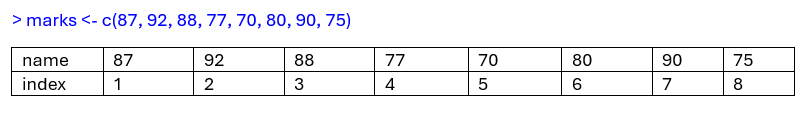
\includegraphics{img/03-index_numeric.png}
\caption{\label{fig:unnamed-chunk-48}Indexing for Numeric Vector}
\end{figure}

\begin{figure}
\centering
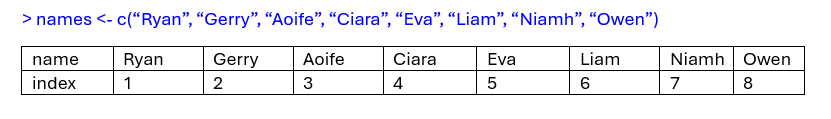
\includegraphics{img/03-index-character.png}
\caption{\label{fig:unnamed-chunk-49}Indexing for Character Vector}
\end{figure}

\begin{figure}
\centering
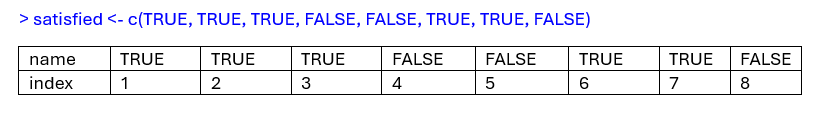
\includegraphics{img/03-index-logical.png}
\caption{\label{fig:unnamed-chunk-50}Indexing for Logical Vector}
\end{figure}

This property in vectors mean we are capable of extracting specific items from a vector based on their position. If I wanted to extract the first item in my list, I can do this by using \texttt{{[}{]}} brackets.

\begin{Shaded}
\begin{Highlighting}[]
\NormalTok{rintro\_names[}\DecValTok{1}\NormalTok{]}
\end{Highlighting}
\end{Shaded}

\begin{verbatim}
## [1] "Gerry"
\end{verbatim}

Similarly, I could extract the 3rd element.

\begin{Shaded}
\begin{Highlighting}[]
\NormalTok{rintro\_marks[}\DecValTok{3}\NormalTok{]}
\end{Highlighting}
\end{Shaded}

\begin{verbatim}
## [1] 87
\end{verbatim}

Or I could extract the last element.

\begin{Shaded}
\begin{Highlighting}[]
\NormalTok{rintro\_satisfied[}\DecValTok{8}\NormalTok{]}
\end{Highlighting}
\end{Shaded}

\begin{verbatim}
## [1] NA
\end{verbatim}

This process is called subsetting. I am taking an original vector and taking a sub-portion of its original elements.

I can ask R even to subset several elements from my vector based on their position. Let's say I want to subset the 2nd, 4th, and 8th elements. I just need to use \texttt{c()} to tell R that I am subsetting several elements.

\begin{Shaded}
\begin{Highlighting}[]
\NormalTok{rintro\_names[}\FunctionTok{c}\NormalTok{(}\DecValTok{2}\NormalTok{, }\DecValTok{4}\NormalTok{, }\DecValTok{8}\NormalTok{)]}
\end{Highlighting}
\end{Shaded}

\begin{verbatim}
## [1] "Aoife" "Eva"   NA
\end{verbatim}

\begin{Shaded}
\begin{Highlighting}[]
\NormalTok{rintro\_marks[}\FunctionTok{c}\NormalTok{(}\DecValTok{2}\NormalTok{, }\DecValTok{4}\NormalTok{, }\DecValTok{8}\NormalTok{)]}
\end{Highlighting}
\end{Shaded}

\begin{verbatim}
## [1] 91 90 NA
\end{verbatim}

\begin{Shaded}
\begin{Highlighting}[]
\NormalTok{rintro\_satisfied[}\FunctionTok{c}\NormalTok{(}\DecValTok{2}\NormalTok{, }\DecValTok{4}\NormalTok{, }\DecValTok{8}\NormalTok{)]}
\end{Highlighting}
\end{Shaded}

\begin{verbatim}
## [1] FALSE FALSE    NA
\end{verbatim}

If the elements you are positioned right next to each other on a vector, you can use \texttt{:} as a shortcut.

\begin{Shaded}
\begin{Highlighting}[]
\NormalTok{rintro\_names[}\FunctionTok{c}\NormalTok{(}\DecValTok{1}\SpecialCharTok{:}\DecValTok{4}\NormalTok{)] }\CommentTok{\#this will extract the elements in index 1, 2, 3, 4}
\end{Highlighting}
\end{Shaded}

\begin{verbatim}
## [1] "Gerry" "Aoife" "Liam"  "Eva"
\end{verbatim}

It's important to know however that when you perform an operation on a vector or you subset it, it does not actually change the original vector. For example, if you wanted to save the top three \texttt{rintro\_marks}, the following code would not work:

\begin{Shaded}
\begin{Highlighting}[]
\FunctionTok{sort}\NormalTok{(rintro\_marks, }\AttributeTok{decreasing =} \ConstantTok{TRUE}\NormalTok{)}


\NormalTok{[}\DecValTok{1}\NormalTok{] }\DecValTok{91} \DecValTok{90} \DecValTok{89} \DecValTok{88} \DecValTok{87} \DecValTok{87}

\NormalTok{rintro\_marks[}\FunctionTok{c}\NormalTok{(}\DecValTok{1}\NormalTok{, }\DecValTok{2}\NormalTok{, }\DecValTok{3}\NormalTok{)]}

\NormalTok{[}\DecValTok{1}\NormalTok{] }\DecValTok{87} \DecValTok{91} \DecValTok{87}

\FunctionTok{print}\NormalTok{(rintro\_marks)}

\NormalTok{[}\DecValTok{1}\NormalTok{] }\DecValTok{87} \DecValTok{91} \DecValTok{87} \DecValTok{90} \DecValTok{88} \DecValTok{89}
\end{Highlighting}
\end{Shaded}

You can see that neither the \texttt{sort()} function or subsetting actually changed the original vector. They just outputted a result to the R console. If I wanted to actually save their results, then I would need to assign them to a variable label.

Here's how I would extract and save the top three exam marks.

\begin{Shaded}
\begin{Highlighting}[]
\NormalTok{marks\_sorted }\OtherTok{\textless{}{-}} \FunctionTok{sort}\NormalTok{(rintro\_marks, }\AttributeTok{decreasing =} \ConstantTok{TRUE}\NormalTok{)}

\NormalTok{marks\_top }\OtherTok{\textless{}{-}}\NormalTok{ marks\_sorted[}\FunctionTok{c}\NormalTok{(}\DecValTok{1}\SpecialCharTok{:}\DecValTok{3}\NormalTok{)]}

\FunctionTok{print}\NormalTok{(marks\_top)}
\end{Highlighting}
\end{Shaded}

\begin{verbatim}
## [1] 91 90 89
\end{verbatim}

Your turn: How could I extract the bottom 3 results? Give it a go.

  \bibliography{book.bib,packages.bib}

\end{document}
